\documentclass[11pt]{article}
\usepackage[T1]{fontenc}
\usepackage{lmodern}
\usepackage[margin=1in]{geometry}
\usepackage{amsmath,amssymb,amsthm,mathtools}
\usepackage{microtype,booktabs,array,longtable}
\usepackage{tikz}
\usetikzlibrary{arrows.meta,positioning,calc}
\usepackage{flafter}
\usepackage[colorlinks=true,linkcolor=blue!50!black,citecolor=blue!50!black,urlcolor=blue!50!black]{hyperref}
\usepackage{bookmark}
\input{glyphtounicode}
\pdfgentounicode=1
\pdfglyphtounicode{tfm:lmex10/parenleftbig}{0028}
\pdfglyphtounicode{tfm:lmex10/parenrightbig}{0029}
\pdfglyphtounicode{tfm:lmex10/vextendsingle}{007C}
\pdfglyphtounicode{tfm:lmex10/vextenddouble}{2225}
\pdfglyphtounicode{tfm:lmex10/parenleftBig}{0028}
\pdfglyphtounicode{tfm:lmex10/parenrightBig}{0029}
\pdfglyphtounicode{tfm:lmex10/parenleftbigg}{0028}
\pdfglyphtounicode{tfm:lmex10/parenrightbigg}{0029}
\pdfglyphtounicode{tfm:lmex10/bracketleftbigg}{005B}
\pdfglyphtounicode{tfm:lmex10/bracketrightbigg}{005D}
\pdfglyphtounicode{tfm:lmex10/floorleftbigg}{230A}
\pdfglyphtounicode{tfm:lmex10/floorrightbigg}{230B}
\pdfglyphtounicode{tfm:lmex10/parenleftBigg}{0028}
\pdfglyphtounicode{tfm:lmex10/parenrightBigg}{0029}
\pdfglyphtounicode{tfm:lmex10/summationtext}{2211}
\pdfglyphtounicode{tfm:lmex10/summationdisplay}{2211}
\pdfglyphtounicode{tfm:lmex10/productdisplay}{220F}
\pdfglyphtounicode{tfm:lmex10/integraldisplay}{222B}
\pdfglyphtounicode{tfm:lmex10/bracketleftBig}{005B}
\pdfglyphtounicode{tfm:lmex10/bracketrightBig}{005D}
\pdfglyphtounicode{tfm:lmex10/ceilingleftBig}{2308}
\pdfglyphtounicode{tfm:lmex10/ceilingrightBig}{2309}
\pdfglyphtounicode{tfm:lmex10/radicalbig}{221A}
\pdfglyphtounicode{tfm:lmex10/radicalBig}{221A}
\pdfglyphtounicode{tfm:lmex10/parenlefttp}{239B}
\pdfglyphtounicode{tfm:lmex10/parenrighttp}{239E}
\pdfglyphtounicode{tfm:lmex10/bracelefttp}{23A7}
\pdfglyphtounicode{tfm:lmex10/braceleftbt}{23A9}
\pdfglyphtounicode{tfm:lmex10/braceleftmid}{23A8}
\pdfglyphtounicode{tfm:lmex10/braceex}{23AA}
\pdfglyphtounicode{tfm:lmex10/parenleftbt}{239D}
\pdfglyphtounicode{tfm:lmex10/parenrightbt}{23A0}
\pdfglyphtounicode{tfm:lmsy10/mapsto}{007C}
\pdfglyphtounicode{tfm:rm-lmr10/Delta}{0394}
\pdfglyphtounicode{tfm:msbm10/C}{2102}
\pdfglyphtounicode{tfm:msbm10/E}{1D53C}
\pdfglyphtounicode{tfm:msbm10/R}{211D}
\pdfglyphtounicode{tfm:msbm10/Z}{2124}
\pdfglyphtounicode{tfm:lmsy10/C}{1D49E}
\pdfglyphtounicode{tfm:lmsy10/E}{2130}
\pdfglyphtounicode{tfm:lmsy10/G}{1D4A2}
\pdfglyphtounicode{tfm:lmsy10/H}{210B}
\pdfglyphtounicode{tfm:lmsy10/K}{1D4A6}
\pdfglyphtounicode{tfm:lmsy10/V}{1D4B1}
\pdfglyphtounicode{tfm:lmsy8/V}{1D4B1}

\pdfinfoomitdate=1
\pdftrailerid{}
\pdfsuppressptexinfo=15
\hypersetup{pdftitle={The periodic spin-one Haldane gap},pdfauthor={OpenAI},bookmarksdepth=2}
\setcounter{tocdepth}{1}
\newtheorem{theorem}{Theorem}[section]
\newtheorem{lemma}[theorem]{Lemma}
\newtheorem{proposition}[theorem]{Proposition}
\newtheorem{corollary}[theorem]{Corollary}
\theoremstyle{definition}
\newtheorem{definition}[theorem]{Definition}
\theoremstyle{remark}
\newtheorem{remark}[theorem]{Remark}
\newcommand{\C}{\mathbb C}
\newcommand{\R}{\mathbb R}
\newcommand{\Z}{\mathbb Z}
\newcommand{\N}{\mathbb N}
\newcommand{\cH}{\mathcal H}
\DeclareMathOperator{\Tr}{Tr}
\DeclareMathOperator{\tr}{tr}
\DeclareMathOperator{\spec}{spec}
\newcommand{\norm}[1]{\left\lVert #1\right\rVert}
\newcommand{\abs}[1]{\left\lvert #1\right\rvert}
\numberwithin{equation}{section}
\setlength{\emergencystretch}{2em}
\title{The periodic spin-one Haldane gap}
\author{OpenAI}
\date{September 24, 2026}
\begin{document}
\maketitle
\begin{abstract}
We prove a uniform positive spectral gap for the pure antiferromagnetic
spin-one Heisenberg chain on even periodic rings, establishing the
positive even-periodic formulation of the spin-one Haldane conjecture.
\end{abstract}
\tableofcontents
\clearpage
\section{Introduction}\label{sec:introduction}

Haldane predicted that antiferromagnetic Heisenberg chains have different
low-energy behavior for integer and half-odd-integer spins. The prediction
was first formulated in 1981 and published in 1983
\cite{Haldane1981,Haldane1983PRL,Haldane1983PLA}. For spin one, the prediction is a
positive gap above the ground energy. We prove this prediction for the
pure bilinear model on even periodic rings, with explicit bounds uniform
in the length.

Let $S^x,S^y,S^z\in M_3(\C)$ be the self-adjoint irreducible spin-one
matrices, normalized by
\[
 [S^\alpha,S^\beta]
   =i\sum_\eta\varepsilon_{\alpha\beta\eta}S^\eta,
 \qquad \sum_\alpha(S^\alpha)^2=2I_3.
\]
For each even integer $L\ge4$, let $\cH_L=(\C^3)^{\otimes L}$ and define
\begin{equation}\label{eq:main-H}
 H_L=\sum_{j=0}^{L-1}\sum_{\alpha=x,y,z}
       S_j^\alpha S_{j+1}^\alpha,
 \qquad S_L^\alpha=S_0^\alpha.
\end{equation}
Here $S_j^\alpha$ acts on site $j$ and is the identity on the other
factors. The coupling constant is one. Write $E_0(L)$ for the least
energy and $E_1(L)$ for the next \emph{distinct} energy of $H_L$, and set
\begin{equation}\label{eq:main-gap}
 \gamma_L=E_1(L)-E_0(L),
 \qquad
 \Delta_1=\liminf_{\substack{L\to\infty\\L\text{ even}}}\gamma_L.
\end{equation}
These definitions concern the full spectrum, including the multiplicity
of the ground energy. The next distinct energy exists: the all-zero and
all-$+1$ product vectors in the $S^z$ basis have energy expectations
$0$ and $L$, respectively, so $H_L$ is not scalar.

\begin{theorem}\label{thm:main}
For the Hamiltonians \eqref{eq:main-H}, the ground state is unique for
every even $L\ge60$, and
\begin{align}
 \gamma_L&>\frac4{105}\log\frac{80}{79}
     &&\text{for every even }L\ge60,\label{eq:gap60}\\
 \gamma_L&>\frac{\log20}{784}
     &&\text{for every even }L\ge2304.\label{eq:gap2304}
\end{align}
Consequently
\[
 \Delta_1\ge\frac{\log20}{784}>0.
\]
The spectral conclusions also hold for any simultaneously similar
spin-one realization satisfying the same commutator and Casimir
normalizations.
\end{theorem}

Theorem~\ref{thm:main} resolves the spin-one Haldane gap conjecture
positively in the even-periodic finite-volume formulation
$\Delta_1>0$. It also implies $\inf_{L\ge4,\,L\text{ even}}\gamma_L>0$:
each of the finitely many remaining finite-dimensional Hamiltonians has
a positive gap above its full ground sector. This observation supplies
neither a numerical value nor a simplicity assertion at those small
lengths.
Corollary~\ref{cor:local-limit} also gives the corresponding lower bound
for local excitations in every subsequential thermodynamic limit of the
periodic ground states of the self-adjoint model.

\subsection{Historical context}

The half-odd-integer side has a rigorous antecedent in the low-energy
excitation bound of Lieb, Schultz and Mattis for the cyclic spin-one-half
chain~\cite[Appendix~B, Theorem~2]{LiebSchultzMattis1961}.
Affleck and Lieb extended this obstruction to the half-odd-integer
antiferromagnetic chains they studied~\cite{AffleckLieb1986}. The possible alternative of degenerate
ground states is part of that obstruction. Integer spin permits a unique
gapped state, but this distinction alone does not prove a gap for a
particular interaction.

The Affleck--Kennedy--Lieb--Tasaki construction established a rigorous
gapped spin-one chain with a biquadratic interaction
\cite{AKLT1987,AKLT1988}. Its bond interaction is
$h+\tfrac13h^2$, up to a scalar and normalization, where
$h=\mathbf S_j\cdot\mathbf S_{j+1}$. The Hamiltonian in
\eqref{eq:main-H} has bond interaction $h$ itself.
Yarotsky proved that a unique ground state and a uniform periodic gap
persist under sufficiently small translation-invariant finite-range
perturbations of the AKLT interaction
\cite[arXiv v1, Theorems~1 and~3]{Yarotsky2006}.
This controls a neighborhood of that interaction; it does not establish
a gapped path to the pure bilinear point.

For the pure spin-one chain, White and Huse's density-matrix
renormalization-group study
estimated a bulk gap of $0.41050(2)$ and exhibited effective spin-one-half
degrees of freedom at open ends~\cite{WhiteHuse1993}. Neutron scattering
provided experimental evidence in the nearly one-dimensional spin-one
antiferromagnet $\mathrm{CsNiCl}_3$~\cite{Buyers1986}.
These results explain both the strong
physical evidence for the prediction and the significance of boundary
conditions. The uniform lower bounds below instead follow from the
stated finite certificates and an analytic argument valid at every
larger even length.

Batista and Ortiz proposed a spin--fermion proof of the Haldane gap
\cite{BatistaOrtiz2001}. Their gap argument following Equation~(8) of the preprint version
uses a first-order perturbative identification with an XYZ chain;
that step does not supply a uniform remainder estimate or a continuation
to the original pairing coefficient. More recently, Tasaki established
a nontrivial infinite-chain topological index for the spin-one
Heisenberg model under a gap assumption for odd open chains with endpoint fields
\cite[arXiv v4, Assumption~2 and Theorem~3]{Tasaki2025}.
The boundary hypotheses of that theorem require a separate argument
from the even-periodic estimates proved here.

Finite-volume methods for uniform spectral gaps have a substantial
history, including the criteria of Knabe and Nachtergaele for
frustration-free chains, whose ground states minimize every local
interaction \cite{Knabe1988,Nachtergaele1996}.
Gosset and Mozgunov obtained sharper finite-size thresholds within that
frustration-free setting~\cite{GossetMozgunov2016}.
Recently, Banerjee, Guo and Chowdhury developed semidefinite bounds for
string correlators using an enclosing ground-energy window, including
finite periodic spin-one Heisenberg chains
\cite[Equations~(2), (13) and Figure~4]{BanerjeeGuoChowdhury2026}.
Those observable bounds concern a different quantity from the uniform
spectral gap studied here.
Our finite inputs are thermal traces of small twisted chains and
variational energy estimates from periodic matrix-product vectors, in the
tradition of finitely correlated states \cite{FNW1992}.
The latter use the standard trace-of-matrix-products representation
\cite[Section~2.1]{PerezGarcia2007}; we give the particular integer
matrices and all contractions explicitly.

The finite thermal inputs are rigorous enclosures of matrix-exponential
traces. Validated matrix exponentiation has a long history, including
self-validating Pad\'e methods~\cite{BochevMarkov1989} and interval
polynomial evaluation~\cite{GoldsztejnNeumaier2014}. Our particular
implementation uses a conditioned Poisson polynomial in a contraction.
The factor-two conditioning estimate follows the coefficient argument
of Fox and Glynn~\cite[Proposition~1]{FoxGlynn1988}. Explicit bounds
for the integer evaluation and the final trace enclosure are supplied
in the appendices.

\subsection{How the proof works}

Quantum transfer-matrix methods relate partition functions to spatial
moments~\cite{Suzuki1985}. Our construction uses an ordered bond
expansion of the type developed by Aizenman and
Nachtergaele~\cite[arXiv v1, Section~2.2]{AizenmanNachtergaele1994}, followed by a
direct operator construction on bond histories.

A shifted partition function is a sum of positive physical Boltzmann
weights. We construct a self-adjoint spatial transfer operator whose
$L$th moment is the same partition function. For even $L$, the spatial
moment is also a sum of nonnegative weights. This gives two probability
distributions associated with one partition function. The \emph{purity}
of a distribution $(p_i)$ is $\sum_i p_i^2$; purity close to one means
that a single weight carries almost all of its mass.

Squaring and renormalizing a distribution reduces its purity defect
quadratically once the defect is small. Squaring physical weights
doubles inverse temperature, while squaring spatial weights doubles
length. Exact cancellation identities couple these two improvements.
Starting from two finite purity bounds, both defects then decay doubly
exponentially as length and inverse temperature double together.
Spatial moment inequalities cover every intermediate even length.
Finally, purity of the full physical Gibbs distribution bounds each
excited-to-ground probability ratio and hence the physical energy gap.
Proposition~\ref{prop:bootstrap} states this coupled argument as a general
gap criterion. Its assumptions isolate a reusable criterion
for other Hamiltonian families with the same two partition-function
representations; positivity of the spatial transfer is not required.

There are two finite initializations. One starts the iteration at length
$60$ and inverse temperature $105/4$. The other reaches length $2304$
and inverse temperature $784$ with a smaller purity defect, giving the
stronger eventual bound. They share the transfer construction and the
bootstrap, while using different thermal moments and two lengths of one
matrix-product trial family.
The finite computations involve integer arithmetic, rational interval
bounds and explicit truncation errors; no floating-point eigenvalue
estimate is a premise.

Section~\ref{sec:model} fixes the model and proves its elementary energy
bounds. Section~\ref{sec:transfer} constructs the spatial transfer and
its rotation sectors. Section~\ref{sec:bootstrap} proves the common
purity theorem, and Section~\ref{sec:initialization} establishes the
two finite initializations from explicitly stated thermal and trial
inputs. Section~\ref{sec:assembly} combines these results to prove
Theorem~\ref{thm:main}. Appendices~\ref{sec:thermal120}--\ref{sec:trials}
prove the essential thermal and trial inputs, with exact data and
reproducible finite procedures.

\section{The Hamiltonian and its auxiliary twists}\label{sec:model}

The argument uses the same partition function in two different ways: as
a Gibbs trace in the physical Hilbert space and as a moment of a spatial
operator. We first choose coordinates that make both descriptions explicit.
We also establish an elementary energy bound used to control the finite
exponential approximations.

\subsection{Spin coordinates}

We use the self-adjoint spin-one matrices. This convention does not restrict
the spectrum in the formulation where self-adjointness is not assumed.

\begin{lemma}[Choice of representation]\label{lem:representation}
Let $S^x,S^y,S^z\in M_3(\C)$ satisfy
\[
 [S^\alpha,S^\beta]
   =i\sum_\gamma\varepsilon_{\alpha\beta\gamma}S^\gamma,
 \qquad \sum_\alpha(S^\alpha)^2=2I.
\]
They are simultaneously similar to the standard self-adjoint spin-one
matrices. If the original matrices are self-adjoint, the similarity can be
chosen unitary. The corresponding tensor-power similarity preserves the
complete spectrum of every periodic Hamiltonian $H_n$.
\end{lemma}

\begin{proof}
Put $S^\pm=S^x\pm iS^y$. The assumptions give
\begin{equation}\label{eq:ladder-identities}
 [S^z,S^\pm]=\pm S^\pm,\qquad
 S^-S^+=2I-(S^z)^2-S^z,\qquad
 S^+S^-=2I-(S^z)^2+S^z.
\end{equation}
Choose an $S^z$ eigenvector $v$ whose eigenvalue $m$ has maximal real part.
Then $S^+v=0$, since otherwise it has eigenvalue $m+1$. Thus $m=1$ or
$m=-2$. The latter case would permit indefinite nonzero lowering: a last
nonzero lowered vector would have weight $-2-k$, whereas
$S^+S^-w=0$ forces its weight to be $-1$ or $2$. This contradicts finite
dimension. Hence $m=1$.

The vectors
\[
 v,\qquad \frac{S^-v}{\sqrt2},\qquad \frac{(S^-)^2v}{2}
\]
are nonzero by \eqref{eq:ladder-identities} and have distinct weights
$1,0,-1$. They form a basis. There is no further lowered vector, because
the basis has no weight $-2$. The identities give raising and lowering
coefficients $\sqrt2$, so this is the standard spin-one representation.
If the original matrices are self-adjoint and $\norm v=1$, the three
vectors are orthonormal. Finally, conjugating each tensor factor conjugates
every term of $H_n$.
\end{proof}

In the weight basis $|s\rangle$, $s\in\{-1,0,1\}$, the diagonal generator
is $S^z|s\rangle=s|s\rangle$ and the nonzero ladder entries are $\sqrt2$.
We will also use the Cartesian basis, indexed by the three axes, in which
\[
 (S^\alpha)_{ij}=-i\varepsilon_{\alpha i j},\qquad
 G_\alpha=iS^\alpha.
\]
These matrices satisfy the same relations. Each $G_\alpha$ is real and
has operator norm one. For the two-site interaction
$h=\sum_\alpha S^\alpha\otimes S^\alpha$, contraction of the epsilon
tensors gives
\begin{equation}\label{eq:cartesian-bond}
 -h=\sum_\alpha G_\alpha\otimes G_\alpha,
 \qquad h=F-|\Omega\rangle\langle\Omega|,
 \qquad \Omega=\sum_{i=1}^3|ii\rangle,
\end{equation}
where $F(u\otimes v)=v\otimes u$. In particular, $h$ has eigenvalues
$-2,-1,1$, and $h\le I$.

\subsection{Twists and partition functions}

Number the sites $0,\ldots,n-1$, with $n\ge4$. A proper Cartesian rotation
$g\in SO(3)$ is unitary on $\C^3$. Define
\begin{equation}\label{eq:twisted-hamiltonian}
 H_n(g)=\sum_{j=0}^{n-2}h_{j,j+1}+h_{n-1,0}(g),
 \qquad
 h_{n-1,0}(g)=\sum_\alpha
 S_{n-1}^\alpha(gS^\alpha g^{-1})_0.
\end{equation}
Thus only the last bond is conjugated, on its site-$0$ factor. The
Hamiltonian is self-adjoint, and $H_n(I)=H_n$. Fix
\begin{equation}\label{eq:shift}
 a=\frac{700741}{500000},\qquad
 Z_n(b,g)=\Tr\exp[-b(H_n(g)+anI)],\qquad Z_n(b)=Z_n(b,I)
 \quad (b>0).
\end{equation}
All these partition functions are strictly positive. The scalar shift
will cancel from the purity ratios and from the final spectral gap.
With this normalization, the trial bounds in Lemma~\ref{lem:trial-inputs}
give $E_0(n)+an<0$ at $n=72,120$, and hence $Z_n(b)>1$ for every $b>0$.
These lower bounds are paired with finite thermal upper bounds in
Section~\ref{sec:initialization}.

We need the diagonal rotations
\[
 P_x=\operatorname{diag}(1,-1,-1),\quad
 P_y=\operatorname{diag}(-1,1,-1),\quad
 P_z=\operatorname{diag}(-1,-1,1),\qquad
 D_2=\{I,P_x,P_y,P_z\},
\]
and the cyclic rotation $C:e_x\mapsto e_y\mapsto e_z\mapsto e_x$.
Write $P=P_x$. The three nonidentity elements of $D_2$ have equal
partition functions, by a global cyclic rotation of all sites. The
rotation $C$ has angle $2\pi/3$ about the diagonal axis. After a global
rotation and a change to the weight basis, $P$ and $C$ are respectively
represented by $\exp(-i\theta S^z)$ with $\theta=\pi$ and
$\theta=2\pi/3$.

For later comparison with finite matrices, a word $x=(x_0,\ldots,x_{n-1})$
in the weight basis has diagonal entry $\sum_j x_{j-1}x_j$, with indices
modulo $n$. Each permitted step changing two neighboring letters by
opposite units has coefficient one. For a seam step from column $y$ to
row $x$, this coefficient is
\begin{equation}\label{eq:seam-phase}
 \exp\bigl(i\theta(y_0-x_0)\bigr).
\end{equation}
Indeed $gS^\pm g^{-1}=e^{\mp i\theta}S^\pm$. These formulas identify the
finite matrices used below with the physical Hamiltonians in
\eqref{eq:twisted-hamiltonian}.

\subsection{A uniform energy bound}

\begin{lemma}[Energy bounds]\label{lem:energy}
For every $n\ge4$ and every $g\in SO(3)$,
\begin{equation}\label{eq:energy-bounds}
 -\frac{3n}{2}I\le H_n(g)\le nI.
\end{equation}
\end{lemma}

\begin{proof}
The upper bound follows from $h\le I$ and unitary conjugation of the
seam. For the lower bound, consider $T=-h_{12}-h_{23}$ on three open
sites in Cartesian coordinates. By \eqref{eq:cartesian-bond}, an unequal
pair swaps with coefficient $-1$, and an equal pair changes to either of
the other equal pairs with coefficient $1$. There are no diagonal terms.

Assign a positive weight $q$ to each three-letter word. The following
table lists every equality pattern; $a,b,c$ denote distinct letters.
The last column sums the weights of the neighbors of a row word, with
the absolute matrix coefficients.
\begin{center}
\begin{tabular}{c|c|c}
word type & $q$ & absolute weighted row sum\\ \hline
$aaa$ & $4$ & $3+3+3+3=12$\\
$aab$ or $abb$ & $3$ & $4+3+2=9$\\
$aba$ & $2$ & $3+3=6$\\
$abc$ & $2$ & $2+2=4$
\end{tabular}
\end{center}
Every row sum is at most $3q$. If $D$ is the diagonal matrix of these
weights, $D^{-1}TD$ has absolute row sums at most three. Its spectral
radius is therefore at most three. Since $T$ is self-adjoint and similar
to this matrix, $h_{12}+h_{23}\ge-3I$.

An open triad containing the seam is unitarily equivalent to an
untwisted triad: delete the seam bond and rotate all sites in one of
the two resulting components. The internal interaction of that component
is rotation invariant. Thus the same lower bound holds for every
consecutive pair of bonds in $H_n(g)$. Summing the $n$ triad inequalities
counts each bond twice and proves \eqref{eq:energy-bounds}.
\end{proof}

\section{Partition functions as spatial moments}\label{sec:transfer}

We now construct a self-adjoint spatial operator whose moments are the
partition functions \eqref{eq:shift}. This identity lets even spatial
powers play the same role as positive Gibbs weights. The operator itself
need not be positive.

Let $\mathcal G\subset SO(3)$ be the group of proper signed permutation
matrices. It contains $D_2$ and $C$. For $g\in\mathcal G$, write
\[
 g e_\alpha=\epsilon_g(\alpha)e_{\sigma_g(\alpha)},
 \qquad \epsilon_g(\alpha)\in\{-1,1\}.
\]
Rotation covariance of the Cartesian matrices gives
\begin{equation}\label{eq:rotation-covariance}
 gG_\alpha g^{-1}
   =\epsilon_g(\alpha)G_{\sigma_g(\alpha)}.
\end{equation}

\begin{proposition}[Spatial transfer]\label{prop:transfer}
For each $b>0$ there are a Hilbert space $\mathcal K_b$, a compact
self-adjoint operator $X_b$, and a unitary representation
$g\mapsto U_g$ of $\mathcal G$ commuting with $X_b$, such that
\begin{equation}\label{eq:spatial-trace}
 Z_n(b,g)=\Tr(X_b^nU_g)
 \qquad(n\ge4,\ g\in\mathcal G).
\end{equation}
The operator $X_b$ and the representation commute with complex
conjugation. Moreover $X_b$ is Hilbert--Schmidt, so $X_b^k$ is trace class
for every integer $k\ge2$. If $\lambda_i(b)$ are its nonzero eigenvalues,
counted with multiplicity, then
\begin{equation}\label{eq:spatial-moments}
 \sum_i|\lambda_i(b)|^k<\infty\quad(k\ge2),\qquad
 Z_n(b)=\sum_i\lambda_i(b)^n\quad(n\ge4).
\end{equation}
\end{proposition}

\begin{proof}
\emph{Histories and the kernel.}
A bond history is a finite ordered list
\[
 x=((t_1,\alpha_1),\ldots,(t_k,\alpha_k)),
 \qquad 0<t_1<\cdots<t_k<b,\quad
 \alpha_j\in\{x,y,z\},
\]
including the empty list when $k=0$. Let $\Omega_b$ be the disjoint union
of these labeled simplexes. Give each simplex Lebesgue measure and the
empty history mass one. The resulting measure $\mu$ is finite:
\begin{equation}\label{eq:history-mass}
 \mu(\Omega_b)=\sum_{k=0}^\infty\frac{3^kb^k}{k!}=e^{3b}.
\end{equation}
Set $\mathcal K_b=L^2(\Omega_b,\mu;\C)$.

For two histories $x,y$, merge their labeled times in increasing order
and define $k_b(x,y)$ as the trace of the resulting product of the
matrices $G_\alpha$, with increasing time from left to right. A nonempty
time collision is a null event; set the kernel to zero there. The product
for two empty histories is the identity, so its trace is three.

The kernel is real and has absolute value at most three, since
$\norm{G_\alpha}=1$. Exchanging $x$ and $y$ leaves their merged
chronological list unchanged. Hence $k_b(x,y)=k_b(y,x)$; no reversal of
the matrix product occurs. Its integral operator $K_b$ is therefore
self-adjoint and Hilbert--Schmidt, with
\[
 \norm{K_b}_{\mathrm{HS}}^2\le9\mu(\Omega_b)^2=9e^{6b}.
\]
Define $X_b=e^{-ab}K_b$. Compact self-adjoint spectral theory gives real,
square-summable eigenvalues. Since they are bounded, all their absolute
moments of integer order at least two are summable. This proves the
operator assertions about $X_b$.

\emph{Rotations.}
The permutation $\sigma_g$ acts on the labels of a history, preserving
its times and the measure. Put
\[
 s_g(x)=\prod_{\alpha\text{ in }x}\epsilon_g(\alpha),\qquad
 (U_g f)(x)=s_g(\sigma_g^{-1}x)f(\sigma_g^{-1}x).
\]
The rule
$s_{gh}(x)=s_g(\sigma_hx)s_h(x)$ proves that these real unitaries form a
representation. Simultaneously rotating every matrix inside a site
trace, using \eqref{eq:rotation-covariance}, gives
\[
 k_b(\sigma_gx,\sigma_gy)=s_g(x)s_g(y)k_b(x,y).
\]
It follows that $U_g$ commutes with $K_b$ and $X_b$. In particular the
kernel of $K_bU_g$ is
\begin{equation}\label{eq:twisted-kernel}
 (K_bU_g)(x,y)=k_b(x,\sigma_gy)s_g(y).
\end{equation}

\emph{The cycle trace.}
For $n\ge2$, both $K_b^{n-1}$ and $K_bU_g$ are Hilbert--Schmidt.
The kernel of $K_b^{n-1}$ is the iterated kernel obtained by integration;
it is bounded because $k_b$ is bounded and $\mu$ is finite. The
Hilbert--Schmidt product trace identity
\[
 \Tr(AB)=\int a(x,y)b(y,x)\,d\mu(x)\,d\mu(y)
\]
and \eqref{eq:twisted-kernel} consequently give
\begin{equation}\label{eq:cycle-integral}
 \Tr(K_b^nU_g)=
 \int_{\Omega_b^n}
 \left(\prod_{j=0}^{n-2}k_b(x_j,x_{j+1})\right)
 k_b(x_{n-1},\sigma_gx_0)s_g(x_0)\,d\mu^n.
\end{equation}
The product trace identity follows from the Hilbert--Schmidt inner
product formula and Cauchy--Schwarz. All the iterated kernel integrals
here are absolutely integrable. Thus \eqref{eq:cycle-integral} does not
require a diagonal-kernel formula for $K_b$ itself.

\emph{Identification with the physical partition function.}
The ordered bond expansion is a standard representation of spin
partition functions~\cite[arXiv v1, Section~2.2, Equations~(2.10)--(2.12)]{AizenmanNachtergaele1994}.
We verify it here with the required seam and normalization.
Expand $\exp[-bH_n(g)]$ in its ordered-time series. By
\eqref{eq:cartesian-bond}, each event chooses a bond and one of three
labels, and inserts the corresponding two $G$ factors. At the seam the
site-$0$ factor is rotated as in \eqref{eq:rotation-covariance}.
There are $(3n)^k$ choices at total degree $k$; each tensor operator has
norm at most one. The sum of the absolute traced contributions is bounded
by
\begin{equation}\label{eq:history-absolute}
 3^n\sum_{k=0}^\infty\frac{(3nb)^k}{k!}=3^ne^{3nb}.
\end{equation}
We may therefore regroup all terms and integrals by bond. The
interleavings of the bond histories partition the global time simplex
up to null collisions. At each site, the tensor trace is the kernel on
the two incident histories, in their original chronological order.

For an explicit check of the seam, call its history $e_0$ and enumerate
the remaining bond histories $e_1,\ldots,e_{n-1}$ around the ring. The
physical integrand is
\[
 s_g(e_0)k_b(\sigma_ge_0,e_1)
 k_b(e_1,e_2)\cdots k_b(e_{n-1},e_0).
\]
In \eqref{eq:cycle-integral}, set
$x_0=e_0,x_1=e_{n-1},\ldots,x_{n-1}=e_1$ and use kernel symmetry.
This gives exactly the displayed integrand, with $g$ on site $0$.
The spatial enumeration has been reversed; the chronological products
have not. Thus $\Tr e^{-bH_n(g)}=\Tr(K_b^nU_g)$. Multiplication by
$e^{-abn}$ proves \eqref{eq:spatial-trace}. The ordinary trace formula
for a compact self-adjoint operator now gives
\eqref{eq:spatial-moments}.
\end{proof}

For an even $n\ge4$, Proposition~\ref{prop:transfer} supplies the
probabilities
\begin{equation}\label{eq:spatial-probabilities}
 p_i=\frac{|\lambda_i(b)|^n}{Z_n(b)},\qquad
 \sum_i p_i=1,\qquad
 \sum_i p_i^2=\frac{Z_{2n}(b)}{Z_n(b)^2}.
\end{equation}
Odd moments will also be useful in polynomial estimates, but evenness is
essential in \eqref{eq:spatial-probabilities}. These spatial eigenvalues
are distinct objects from the physical energies of $H_n$.

\subsection{Rotation sectors}

The small twisted partition functions separate the spatial eigenvalues
into a few lists. Their multiplicities will help isolate a dominant
weight; no restriction on the physical spectrum is imposed.

\begin{lemma}[Sector moments]\label{lem:sectors}
Fix $b>0$ and let $X_b,U_g$ be as in Proposition~\ref{prop:transfer}.
There are real eigenvalue lists, counted with multiplicity, whose
integer moments $I_k,O_k,N_k$ converge absolutely for $k\ge2$, with
\begin{align}
 Z_n(b)&=I_n+2O_n+3N_n,\label{eq:sector-total}\\
 Z_n(b,P)&=I_n+2O_n-N_n,\label{eq:sector-pi}\\
 Z_n(b,C)&=I_n-O_n\qquad(n\ge4).\label{eq:sector-cyclic}
\end{align}
The $I$ list is the restriction to the joint invariant subspace of
$D_2$ and $C$. The $O$ list occurs twice and the $N$ list three times
in the full eigenvalue list of $X_b$. All three moments are nonnegative
at even orders. If $J_n$ denotes the moment on the $D_2$-invariant
subspace, then
\[
 J_n=I_n+2O_n.
\]
\end{lemma}

\begin{proof}
The four characters $\chi$ of $D_2$ define orthogonal projections
\[
 \Pi_\chi=\frac14\sum_{g\in D_2}\chi(g)U_g.
\]
They commute with $X_b$ and sum to the identity. Conjugation by $U_C$
permutes the three nontrivial character spaces cyclically. The
restrictions of $X_b$ to these spaces are therefore unitarily equivalent;
denote their common moment by $N_k$.

In the trivial-character space, split further according to the
eigenvalues $1,\omega,\overline\omega$ of $U_C$, where
$\omega=e^{2\pi i/3}$. These are reducing subspaces for $X_b$. Complex
conjugation exchanges the last two spaces and preserves every real
eigenvalue of $X_b$, with multiplicity. Their common moment is $O_k$;
the moment on the first space is $I_k$. Absolute convergence follows
from \eqref{eq:spatial-moments}.

This orthogonal decomposition proves \eqref{eq:sector-total}. On the
three nontrivial character spaces, a fixed $U_P$ has signs $+1,-1,-1$,
while it is the identity on the trivial-character space. This gives
\eqref{eq:sector-pi}. The operator $U_C$ permutes the nontrivial spaces,
so they contribute zero to $\Tr(X_b^nU_C)$. On the remaining three
spaces its coefficients are $1,\omega,\overline\omega$, and
$\omega+\overline\omega=-1$. This proves
\eqref{eq:sector-cyclic}. The identity for $J_n$ follows from the
decomposition of the trivial-character space; even powers give nonnegativity.
\end{proof}

The invariant $I$ space need not be one-dimensional. The point of
Lemma~\ref{lem:sectors} is that every weight outside it occurs at least
twice in the full list. Later moment bounds will identify a unique
largest weight without discarding any sector.

\section{From two purities to a uniform gap}\label{sec:bootstrap}

The spatial and physical descriptions of the same partition function
give two ways to concentrate its weights.  This section isolates the
argument that propagates two initial concentration estimates to all
larger even lengths.  The initial estimates are established in
Section~\ref{sec:initialization}.

By Proposition~\ref{prop:transfer}, each partition function is both a
physical Gibbs trace and, at even lengths, a nonnegative spatial moment.
The former counts every physical eigenvector, with multiplicity; the
latter counts the absolute powers of every spatial eigenvalue. These
two representations give the two probability distributions used below.

For even $n\ge4$, define the spatial and physical purities
\begin{equation}\label{eq:purities}
 S(n,b)=\frac{Z_{2n}(b)}{Z_n(b)^2},\qquad
 T(n,b)=\frac{Z_n(2b)}{Z_n(b)^2}.
\end{equation}
The energy shift $aL$ cancels from both ratios.  We first record the
elementary inequality responsible for their improvement under squaring.

\begin{lemma}[Squaring probabilities]\label{lem:purity}
Let $(w_i)$ be a finite or countable family of nonnegative numbers with
$\sum_iw_i=1$. Its purity $P=\sum_iw_i^2$ lies in $(0,1]$.
The normalized squares $w_i^2/P$ have purity $P'$ satisfying
\begin{equation}\label{eq:purity-square}
 1-P'\le f(1-P),\qquad
 f(u)=\frac{u^2}{2(1-u)^2}\quad(0\le u<1).
\end{equation}
The function $f$ is increasing.  Consequently
\begin{equation}\label{eq:two-squarings}
 \begin{split}
 0<S(n,b),T(n,b)&\le1,\\
 1-S(2n,b)&\le f(1-S(n,b)),\\
 1-T(n,2b)&\le f(1-T(n,b)).
 \end{split}
\end{equation}
\end{lemma}

\begin{proof}
At least one weight is positive, so $P>0$, and $w_i^2\le w_i$ gives
$P\le1$. Nonnegativity permits rearrangement of all countable sums.
Thus
\[
 1-P'
 =\frac{2\sum_{i<j}w_i^2w_j^2}{P^2}
 \le\frac{2\bigl(\sum_{i<j}w_iw_j\bigr)^2}{P^2}
 =\frac{(1-P)^2}{2P^2}.
\]
Also $f'(u)=u/(1-u)^3\ge0$.

For $S(n,b)$, use the spatial probabilities
$|\lambda_i(b)|^n/Z_n(b)$ from \eqref{eq:spatial-probabilities}.
Squaring them changes $n$ to $2n$. For $T(n,b)$, list all physical
eigenvalues $\varepsilon_k(n)$ with multiplicity and use
\begin{equation}\label{eq:gibbs-weights}
 w_k(n,b)=\frac{e^{-b(\varepsilon_k(n)+an)}}{Z_n(b)}.
\end{equation}
Their purity is $T(n,b)$, and squaring them changes $b$ to $2b$.
This proves \eqref{eq:two-squarings}.
\end{proof}

\subsection{The coupled update}

The two purities constrain one another because their definitions use
the same partition functions.  Direct cancellation gives
\begin{align}
 S(n,2b)&=S(n,b)^2\frac{T(2n,b)}{T(n,b)^2},
   \label{eq:space-time-cancel}\\
 T(4n,b)&=T(2n,b)^2\frac{S(2n,2b)}{S(2n,b)^2}.
   \label{eq:time-space-cancel}
\end{align}
Both denominators are at most one.  The following form allows the
initial bounds to have different sizes and to be rounded upward.

\begin{lemma}[Coupled update]\label{lem:rounded-update}
Suppose $n\ge4$ is even, $b>0$, and $p,q\in[0,1)$ satisfy
\[
 1-S(n,b)\le p,\qquad 1-T(2n,b)\le q.
\]
If $p_+,q_+\in[0,1)$ obey
\begin{equation}\label{eq:rounded-update}
 \begin{split}
 p_+&\ge f\bigl(1-(1-p)^2(1-q)\bigr),\\
 q_+&\ge f\bigl(1-(1-q)^2(1-p_+)\bigr),
 \end{split}
\end{equation}
then
\[
 1-S(2n,2b)\le p_+,\qquad
 1-T(4n,2b)\le q_+.
\]
\end{lemma}

\begin{proof}
Equation~\eqref{eq:space-time-cancel} gives
$S(n,2b)\ge(1-p)^2(1-q)$. Applying spatial squaring in
Lemma~\ref{lem:purity} and monotonicity of $f$ proves the first bound.
Next \eqref{eq:time-space-cancel} gives
$T(4n,b)\ge(1-q)^2(1-p_+)$. Temporal squaring proves the second.
Every input of $f$ is in $[0,1)$ because the product subtracted from
one is positive and at most one.
\end{proof}

In particular, one may round the first output upward before using it
in the second update, then round the second output upward.  The pair
based at $(n,b)$ becomes a pair based at $(2n,2b)$: its physical member
is at length $4n$.  No decrease of the individual bounds is needed for
this step.

\subsection{Quadratic decay and intermediate lengths}

Once both defects are small, one common bound suffices.  Put
\begin{equation}\label{eq:bootstrap-coefficient}
 G(u)=\frac12\left((1-u)^{-1}+(1-u)^{-2}+(1-u)^{-3}\right)^2.
\end{equation}
This function is increasing on $[0,1)$, and
\begin{equation}\label{eq:bootstrap-factorization}
 f\bigl(1-(1-u)^3\bigr)=G(u)u^2.
\end{equation}

\begin{proposition}[Uniform gap from two initial purities]
\label{prop:bootstrap}
For every even $L\ge4$, let $H_L$ be a non-scalar finite-dimensional
self-adjoint Hamiltonian. Suppose that $a\in\R$ and, for each $b>0$,
a real finite or countable list $(\lambda_i(b))$ satisfy
\[
 \sum_i|\lambda_i(b)|^4<\infty,\qquad
 Z_L(b):=\Tr e^{-b(H_L+aLI)}=\sum_i|\lambda_i(b)|^L
 \quad(L\ge4\text{ even}).
\]
Define $S,T$ by \eqref{eq:purities} and $G$ by
\eqref{eq:bootstrap-coefficient}. Let $n_0\ge4$ be even,
$b_0>0$, and let $u_0,C$ satisfy
\begin{equation}\label{eq:bootstrap-hypotheses}
 0<u_0<\frac16,\qquad G(u_0)\le C,\qquad
 r:=Cu_0<1,\qquad C(1-3u_0)>3.
\end{equation}
Suppose
\begin{equation}\label{eq:bootstrap-seeds}
 S(n_0,b_0)\ge1-u_0,\qquad T(2n_0,b_0)\ge1-u_0.
\end{equation}
For $j\ge0$, set
\begin{equation}\label{eq:dyadic-parameters}
 n_j=2^j n_0,\qquad b_j=2^j b_0,\qquad
 u_j=C^{-1}r^{2^j}.
\end{equation}
Then
\begin{equation}\label{eq:dyadic-purities}
 S(n_j,b_j)\ge1-u_j,\qquad T(2n_j,b_j)\ge1-u_j.
\end{equation}
For every even $L\ge n_0$, the physical ground state is unique, and
the gap above it satisfies
\begin{equation}\label{eq:bootstrap-gap}
 \gamma_L>\frac{\log(1/r)}{b_0}.
\end{equation}
\end{proposition}

\begin{proof}
\emph{Doubling.}
The definition gives $u_{j+1}=Cu_j^2$ and
$0<u_{j+1}<u_j\le u_0$.  Suppose both defects at $(n_j,b_j)$ are at
most $u=u_j$.  The first bound in Lemma~\ref{lem:rounded-update} is at
most
\[
 f\bigl(1-(1-u)^3\bigr)=G(u)u^2\le Cu^2=u_{j+1}\le u.
\]
Use $p_+=u_{j+1}$ in the second update.  Its input is at most
$1-(1-u)^3$, so its output is also at most $Cu^2=u_{j+1}$.
Induction proves \eqref{eq:dyadic-purities}.

\emph{Intermediate even lengths.}
For any nonnegative list $(a_i)$ with finite positive $p$th-power sum
and $q\ge p>0$, normalization gives
\[
 \sum_i a_i^q\le\left(\sum_i a_i^p\right)^{q/p}.
\]
Indeed the normalized $p$th powers are probabilities, whose
$(q/p)$th powers sum to at most one.  Apply this to the absolute spatial
eigenvalues at each of the two temperatures.  Whenever $n\le L\le2n$
and both lengths are even,
\[
 Z_L(b)\le Z_n(b)^{L/n},\qquad
 Z_L(2b)\ge Z_{2n}(2b)^{L/(2n)}.
\]
Combining them yields the interpolation inequality
\begin{equation}\label{eq:purity-interpolation}
 T(L,b)\ge
 \left[T(2n,b)S(n,b)^2\right]^{L/(2n)}.
\end{equation}
The bracket lies in $(0,1]$ and the exponent lies in $[1/2,1]$.
For $n=n_j$ and $b=b_j$, we therefore have
\begin{equation}\label{eq:intermediate-purity}
 T(L,b_j)\ge(1-u_j)^3\ge1-3u_j>\frac12
 \qquad(n_j\le L\le2n_j,\ L\text{ even}).
\end{equation}

\emph{The physical spectrum.}
The largest weight in \eqref{eq:gibbs-weights} is at least its purity,
since $\sum_k w_k^2\le(\max_k w_k)\sum_k w_k$.  It is consequently
greater than $1/2$.  These weights count all physical eigenvectors;
two ground-state eigenvectors would have two equal maximal weights,
which is impossible.  Thus the ground state is unique.

Because $H_L$ is non-scalar and self-adjoint in finite dimension, a
next distinct energy exists.  Let $w_0$ be the ground-state weight and
let $w_1$ be the weight of an eigenvector at that next energy.  Then
\begin{align}
 e^{-b_j\gamma_L}
 &=\frac{w_1}{w_0}
 \le\frac{1-w_0}{w_0}
 \le\frac{3u_j}{1-3u_j}\notag\\
 &\le\frac{3}{C(1-3u_0)}r^{2^j}
 <r^{2^j}.
 \label{eq:gap-ratio}
\end{align}
Here the shift $aL$ cancels, and the final strict inequality follows
from \eqref{eq:bootstrap-hypotheses}. Taking logarithms and using
$b_j=2^j b_0$ proves \eqref{eq:bootstrap-gap} throughout the interval
$n_j\le L\le2n_j$.  These dyadic intervals cover every even
$L\ge n_0$.
\end{proof}

Figure~\ref{fig:bootstrap} summarizes the two operations in the proof:
doubling advances the pair of purity estimates, and interpolation fills
the interval of physical lengths controlled at each temperature.

\begin{figure}[tb]
\centering
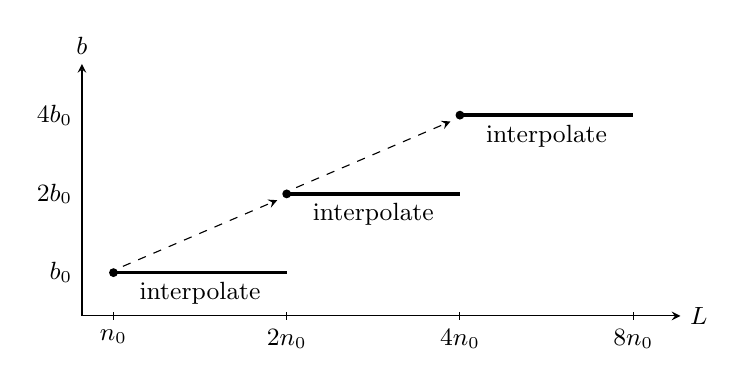
\begin{tikzpicture}[>=stealth, every node/.style={font=\small}]
 \draw[->] (-0.4,-0.55) -- (7.2,-0.55) node[right] {$L$};
 \draw[->] (-0.4,-0.55) -- (-0.4,2.65) node[above] {$b$};
 \foreach \x/\lab in {0/n_0,2.2/2n_0,4.4/4n_0,6.6/8n_0}
   {\draw (\x,-0.5)--(\x,-0.6);
    \node[below] at (\x,-0.6) {$\lab$};}
 \foreach \y/\lab in {0/b_0,1/2b_0,2/4b_0}
   {\node[left] at (-0.4,\y) {$\lab$};}
 \draw[very thick] (0,0)--(2.2,0);
 \draw[very thick] (2.2,1)--(4.4,1);
 \draw[very thick] (4.4,2)--(6.6,2);
 \fill (0,0) circle (1.6pt);
 \fill (2.2,1) circle (1.6pt);
 \fill (4.4,2) circle (1.6pt);
 \draw[->,dashed] (0.12,0.08)--(2.08,0.92);
 \draw[->,dashed] (2.32,1.08)--(4.28,1.92);
 \node[below] at (1.1,0) {interpolate};
 \node[below] at (3.3,1) {interpolate};
 \node[below] at (5.5,2) {interpolate};
\end{tikzpicture}
\caption{The bootstrap, shown schematically at three dyadic scales.
Dashed arrows double the starting length and inverse temperature.
At each scale, interpolation controls the physical purity for every
even length on the solid interval.  The intervals cover all larger
even lengths.}
\label{fig:bootstrap}
\end{figure}

\subsection{The two parameter choices}

We will establish the initial inequalities
\eqref{eq:bootstrap-seeds} for the following two rows:
\begin{equation}\label{eq:bootstrap-parameters}
\begin{array}{c|c|c|c|c}
 n_0&b_0&u_0&C&r=Cu_0\\ \hline
 60&105/4&1/8&79/10&79/80\\
 2304&784&1/100&5&1/20
\end{array}
\end{equation}
The scalar hypotheses of Proposition~\ref{prop:bootstrap} can already
be checked. For the first row,
\[
 G(1/8)=\frac{913952}{117649}<\frac{79}{10},\qquad
 \frac{3}{C(1-3u_0)}=\frac{48}{79}<1.
\]
For the second, $1-(1-u)^3\le3u$ gives, when $0<u\le1/100$,
\[
 G(u)\le\frac{9}{2(1-3u)^2}
 \le\frac{45000}{9409}<5,\qquad
 \frac{3}{C(1-3u_0)}=\frac{60}{97}<1.
\]
Thus the two rows give respectively the bounds
$(4/105)\log(80/79)$ and $(\log20)/784$ in
\eqref{eq:bootstrap-gap}, once their initial purities are proved.
The second row will follow from six applications of
Lemma~\ref{lem:rounded-update} to bounds based at $(36,49/4)$.
The remaining task is therefore finite: establish the two sets of
initial inequalities without losing the margins needed in these
updates.

\section{Two finite initializations}\label{sec:initialization}

The doubling argument requires a spatial purity at length $n$ and a physical
purity at length $2n$, at the same inverse temperature.  We establish two such
pairs.  The first begins at length $60$; the second begins at length $2304$ and
gives the stronger eventual gap.  In both cases the inputs are a few short-chain
partition functions and one periodic trial vector.  This section explains how
those finite inputs imply the required purities.

\subsection{Thermal data and elementary moment bounds}

We use the sectors from Lemma~\ref{lem:sectors}: $J_n=I_n+2O_n$ is the
$D_2$-invariant moment, $I_n$ is the moment fixed also by the cyclic rotation,
and $N_n$ is the moment in one nontrivial $D_2$ sector.  Each $O_n$ occurs twice
and each $N_n$ occurs three times in the full trace.  In particular,
\begin{equation}\label{eq:sector-inversion}
\begin{aligned}
 J_n&=\frac{Z_n+3Z_n(P)}4,&
 N_n&=\frac{Z_n-Z_n(P)}4,\\
 I_n&=\frac{Z_n+3Z_n(P)+8Z_n(C)}{12},&
 O_n&=\frac{Z_n+3Z_n(P)-4Z_n(C)}{12}.
\end{aligned}
\end{equation}
The inverse temperature is common to every term of each identity.

\begin{lemma}[Finite thermal inputs]\label{lem:thermal-inputs}
For $a=700741/500000$, the following tables give centers for the shifted
partition functions $Z_n(b,g)$ in units $10^{-6}$.
The absolute errors are less than $10^{-5}$ at $b=21/2$ and less than
$30\cdot10^{-6}$ at $b=49/4$.
\[
\begin{array}{c|rrr}
 &\multicolumn{3}{c}{b=21/2}\\
 n&g=1&g=P&g=C\\ \hline
 6&8945303&346734&939987\\
 8&3741281&567167&984108\\
 10&2327547&721090&1002613
\end{array}
\qquad
\begin{array}{c|rr}
 &\multicolumn{2}{c}{b=49/4}\\
 n&g=1&g=P\\ \hline
 4&124885379&65757\\
 5&2925&2960742\\
 6&12870614&286599\\
 7&54069&1920414\\
 8&4639283&510140\\
 9&195455&1514846\\
 10&2654823&675419\\
 11&377629&1314544\\
 12&1900547&787405
\end{array}
\]
\end{lemma}

Appendices~\ref{sec:thermal120} and~\ref{sec:thermal72} prove the respective
tables by rational approximations to the physical matrix exponentials,
with explicit error bounds.  Lemma~\ref{lem:trial-inputs} supplies the other
finite input:
\begin{equation}\label{eq:trial-thermal-consequence}
 E_0(72)<-72a,\qquad E_0(120)<-120a.
\end{equation}
Consequently $Z_{72}(b)>1$ and $Z_{120}(b)>1$ for every $b>0$: in each case
one Boltzmann factor already exceeds one.

Here are two elementary ways to extract spectral information from the tables.

\begin{lemma}[Capped masses]\label{lem:cappedmass}
Let $(t_i)$ be a finite or countable family with $0\le t_i\le h$ and
$\sum_i t_i\le m$, where $h>0$ and $m\ge0$.  For $r\ge1$, put
\begin{equation}\label{eq:capped-function}
 \mathcal C(m,h,r)=q h^r+(m-qh)^r,\qquad q=\lfloor m/h\rfloor.
\end{equation}
Then $\sum_i t_i^r\le\mathcal C(m,h,r)$.  Without the individual cap,
$\sum_i t_i^r\le m^r$.
\end{lemma}

\begin{proof}
For a finite family at fixed total mass, transfer mass from the smaller of two
coordinates in $(0,h)$ to the larger until one reaches $0$ or $h$.  Convexity
shows that the sum of $r$th powers does not decrease.  Repetition leaves at most
one coordinate in $(0,h)$, giving~\eqref{eq:capped-function} at the actual
total mass.  That expression is continuous and nondecreasing in the total
mass, so it is bounded by its value at $m$.  Apply this argument to finite
subfamilies and take their increasing union for a countable family.  The
uncapped assertion follows directly from
$t_i^r\le t_i(\sum_jt_j)^{r-1}$ when the total mass is positive; the zero case
is immediate.
\end{proof}

\begin{lemma}[Polynomial filter]\label{lem:polynomial-filter}
Let $\epsilon\ge0$, $v>0$, and let $(\lambda_i)$ be a real eigenvalue list with moments
$M_j=\sum_i\lambda_i^j$, and suppose $|M_j-c_j|\le\epsilon$ for the
indices occurring in a polynomial $F(x)=\sum_j f_jx^j$.
Assume these moments converge absolutely and $F\ge0$ on $\R$.
If
\[
 B=\sum_j f_jc_j+\epsilon\sum_j|f_j|
 \quad\hbox{and}\quad F(x)>B\ \hbox{for }|x|\ge v,
\]
then every $|\lambda_i|<v$.
\end{lemma}

\begin{proof}
Absolute convergence gives $\sum_iF(\lambda_i)\le B$.  Since every summand
is nonnegative, one eigenvalue with $|\lambda_i|\ge v$ would contradict this
bound.
\end{proof}

All moments used below converge absolutely by Proposition~\ref{prop:transfer}.
The coefficient sums in~\eqref{eq:sector-inversion} are at most one in
absolute value, so the thermal error bound also bounds each sector-moment
error.  This observation includes the odd moments used in the second
initialization; their signs are retained in the polynomial filter.

\subsection{The initialization at length sixty}

\begin{proposition}\label{prop:seed60}
At inverse temperature $b=105/4$,
\[
 S(60,b)>\frac78,\qquad T(120,b)>\frac78.
\]
\end{proposition}

\begin{proof}
We first bound sector moments and then increase the inverse temperature.
The trial energy forces a dominant spatial weight, giving the spatial
purity; its physical Boltzmann factor will give the physical purity
separately.

Begin at the lower inverse temperature $b_0=21/2$.  From the $b_0=21/2$ table in
Lemma~\ref{lem:thermal-inputs} and~\eqref{eq:sector-inversion}, upper bounds
for $I_{10},O_{10},N_{10}$ are, respectively,
\[
 m_I=\frac{1042655}{10^6},\qquad
 m_O=\frac{40041}{10^6},\qquad
 m_N=\frac{401625}{10^6}.
\]
For clarity, their margins over the sector centers plus $10^{-5}$ are
$19/(12\cdot10^6)$, $7/(12\cdot10^6)$ and $3/(4\cdot10^6)$.

Apply Lemma~\ref{lem:polynomial-filter} to
\[
 F_I(x)=x^6(-2+10x^2)^2,\qquad
 F_N(x)=x^6(-25+100x^2)^2.
\]
For a filter $x^6(c_0+c_1x^2)^2$, its summed upper bound is the centered
combination of moments $6,8,10$ with coefficients $c_0^2,2c_0c_1,c_1^2$,
plus $10^{-5}(|c_0|+|c_1|)^2$.  Direct rational evaluation gives
\[
 |\lambda|<U:=\frac{100245}{100000}\quad\hbox{in }I,
 \qquad
 |\lambda|<V:=\frac{88643}{100000}\quad\hbox{in }N.
\]
Indeed the filter value at the indicated endpoint exceeds its summed upper
bound by more than $0.0301$ for $I$ and $0.3463$ for $N$.
Each filter is strictly increasing with $|x|$ beyond its endpoint: there
$c_1>0$ and $c_0+c_1x^2>0$.

The rational inequalities
$U^{10}<m_I<2U^{10}$ and $V^{10}<m_N<2V^{10}$ allow the two-piece form
of Lemma~\ref{lem:cappedmass}.  For $k=30,120$ define
\[
 A_k=U^k+(m_I-U^{10})^{k/10},\qquad
 B_k=m_O^{k/10},\qquad
 C_k=V^k+(m_N-V^{10})^{k/10}.
\]
They bound $I_k,O_k,N_k$, respectively.  Because these are even moments,
all are nonnegative, and hence
\begin{equation}\label{eq:short-moment-upper}
 Z_k(b_0)\le A_k+2B_k+3C_k,\qquad
 Z_k(b_0,P),\ Z_k(b_0,C)\le A_k+2B_k.
\end{equation}
Put $m=A_{30}+2B_{30}+3C_{30}$, $p=A_{30}+2B_{30}$, and
$q=A_{120}+2B_{120}+3C_{120}$.  With
\[
 D=\frac{1450}{1000},\quad E=\frac{1202}{1000},\quad
 \tau=\frac{1225}{1000},\quad\tau_0=\frac{1264}{1000},\quad
 R_q=\frac{684}{10000},
\]
the remaining scalar estimates are
\begin{equation}\label{eq:seed60-scalars}
\begin{gathered}
 m^5<D^2,\qquad p^5<E^2,\qquad
 q\ge1,\qquad (q-1)^5<R_q^2,\\
 \frac{D+11E}{12}\le\tau,\qquad
 \frac{D+3E}{4}\le\tau_0.
\end{gathered}
\end{equation}
For example, the positive margins in the first, second and fourth strict
inequalities exceed $0.001068$, $0.000433$ and $0.0000472$, respectively.
Every number in these comparisons is rational and is specified above.

We now increase the inverse temperature from $b_0$ to
$b=(5/2)b_0$.  For positive Boltzmann factors $z_i$,
$\sum_i z_i^{5/2}\le(\sum_i z_i)^{5/2}$.  Thus
\eqref{eq:short-moment-upper}--\eqref{eq:seed60-scalars} imply
\[
 Z_{30}(b)\le D,\qquad Z_{30}(b,P),Z_{30}(b,C)\le E.
\]
By~\eqref{eq:sector-inversion}, the $I$ and $J$ portions of the thirtieth
spatial moment are at most $\tau$ and $\tau_0$.

Let $w_i=|\lambda_i(X_b)|^{30}$.  Then $\sum_iw_i\le D$, whereas
\eqref{eq:trial-thermal-consequence} gives $\sum_iw_i^4=Z_{120}(b)>1$.
Since $D(0.88)^3<1$, some weight $w_0>0.88$ exists.  It is unique because
$2(0.88)>D$.  It belongs to $I$: a weight in $O$ would occur at least twice,
and one in $N$ at least three times.  These statements count all
multiplicities, including equal moduli of opposite-sign spatial eigenvalues.

To sharpen the lower bound on $w_0$, suppose $0\le t\le0.998$ and $w_0\ge t$.
Denote the remaining
$I$ mass by $x$, the full $O$-pair mass by $y$, and the full $N$-triple mass
by $z$.  Their squared weights sum to at most $x^2+y^2/2+z^2/3$, and
\[
 0\le x\le\tau-t,\qquad 0\le y,\qquad
 x+y\le\tau_0-t,\qquad z\le D-t-x-y.
\]
The divisors $2$ and $3$ use the identical weight lists in the repeated
sectors.  Since $D>\tau_0$, the last upper bound is nonnegative on the entire
displayed polygon.  The convex quadratic
$x^2+y^2/2+(D-t-x-y)^2/3$ has its maximum at one of its four vertices.  Write
\begin{equation}\label{eq:residual-R}
 R(t)=\max_{(x,y)\in\mathcal V_t}
 \left(x^2+\frac{y^2}{2}+\frac{(D-t-x-y)^2}{3}\right),
\end{equation}
where
\[
 \mathcal V_t=\{(0,0),(\tau-t,0),
 (\tau-t,\tau_0-\tau),(0,\tau_0-t)\}.
\]
Thus the remaining squared weights sum to at most $R(t)$, and their fourth
powers sum to at most $R(t)^2$.  Exact evaluation gives
\[
\begin{array}{c|ccc}
 t&0.88&0.99&0.998\\ \hline
 R(t)&0.1359&0.0721&0.068404
\end{array}
\]
and
\[
 1-0.99^4-R(0.88)^2=0.02093518,\qquad
 1-0.998^4-R(0.99)^2=0.002777621984.
\]
If $w_0\le0.99$, the first equality would contradict
$\sum_iw_i^4>1$; the second then excludes $w_0\le0.998$.
Keeping the dominant contribution in the fourth moment yields
\[
 S(60,b)=\frac{\sum_iw_i^4}{(\sum_iw_i^2)^2}
 \ge\left(1+\frac{R(0.998)}{0.998^2}\right)^{-2}
 >0.8756>\frac78.
\]

For the physical purity at length $120$, return briefly to temperature $b_0$.
Its largest Boltzmann factor $z_0$ exceeds one by the trial bound, while the
sum of all factors is at most $q$.  After raising the factors to the power
$5/2$, the ratio of the remaining mass to $z_0^{5/2}$ is at most
$(q-1)^{5/2}<R_q$.  Therefore
\[
 T(120,b)\ge(1+R_q)^{-2}>0.8760>\frac78.
\]
This last step concerns physical Boltzmann factors, separately from the
spatial weights used to bound $S$.
\end{proof}

\subsection{The initialization giving the stronger gap}

\begin{proposition}\label{prop:seed2304}
At inverse temperature $b=784$,
\[
 1-S(2304,b)\le\frac{84513}{10^7}<\frac1{100},\qquad
 1-T(4608,b)\le\frac{27493}{5\cdot10^6}<\frac1{100}.
\]
\end{proposition}

\begin{proof}
We isolate one large eigenvalue in $J$ and bound the remaining moments.
This gives a pair of initial purity defects at length $36$; six rounded
updates then reach length $2304$.

Begin at $b_0=49/4$.  The $b_0=49/4$ table gives centers for $J_n,N_n$
through~\eqref{eq:sector-inversion}, with error at most
$\epsilon=30\cdot10^{-6}$.  Use the two filters
\[
 F_J(x)=x^4(7+17x-280x^2-185x^3+1000x^4)^2,
 \qquad F_N(x)=x^4(12-394x^2+1000x^4)^2.
\]
Their degree is $12$, so the table supplies every required moment.  The
summed upper bounds in Lemma~\ref{lem:polynomial-filter} are exactly
\[
 B_J=318604.54848175,\qquad B_N=48169.880699.
\]
Set $v_J=100139/100000$ and $v_N=872/1000$.  Direct rational comparisons give
\[
 F_J(v_J)-B_J>180,\quad F_J(-v_J)-B_J>496888,\quad
 F_N(\pm v_N)-B_N>654.
\]
To check the whole exterior rays without further numerical tests, write
$Q(x)=7+17x-280x^2-185x^3+1000x^4$.  For $y\ge0$,
\[
\begin{aligned}
 Q(1+y)&=559+2902y+5165y^2+3815y^3+1000y^4,\\
 Q(-1-y)&=895+3978y+6275y^2+4185y^3+1000y^4.
\end{aligned}
\]
Both are positive and increasing.  The polynomial
$12-394r^2+1000r^4$ is likewise positive and increasing for $r\ge v_N$:
its value at $v_N$ is positive and its derivative is
$4r(1000r^2-197)>0$.  Thus the filters increase along the requisite rays,
and every eigenvalue has modulus less than $v_J$ in $J$ and less than
$v_N$ in $N$.

The twelfth-moment upper bounds are
\[
 m_J=1.0657205,\qquad m_N=0.2783155.
\]
Put $\ell=999/1000$ and, for $k=36,72$, define
\begin{equation}\label{eq:seed72-tail}
 B(k)=3\mathcal C(m_N,v_N^{12},k/12),\qquad
 R_A(k)=B(k)+(m_J-\ell^{12})^{k/12}.
\end{equation}
Here $m_J>\ell^{12}$.  If all eigenvalues in $J$ had modulus at most $\ell$,
Lemma~\ref{lem:cappedmass} would imply
\[
 Z_{72}(b_0)\le\mathcal C(m_J,\ell^{12},6)+B(72)<1,
\]
where the strict margin to one exceeds $0.0693$.  The trial inequality
contradicts this.  Choose an eigenvalue $\lambda_0$ in $J$ with
$|\lambda_0|>\ell$.  Removing it leaves a twelfth-moment mass at most
$m_J-\ell^{12}$ in $J$.  The uncapped bound of Lemma~\ref{lem:cappedmass}
and the three $N$ sectors show that $R_A(k)$ bounds the remaining full
$k$th moment.

It follows that
\begin{equation}\label{eq:seed72-pq}
\begin{aligned}
 1-S(36,b_0)&\le p_0:=1-\left(1+\frac{R_A(36)}{\ell^{36}}\right)^{-2},\\
 1-T(72,b_0)&\le q_0:=1-\left(v_J^{72}+R_A(72)\right)^{-2}.
\end{aligned}
\end{equation}
For the first estimate retain $\lambda_0^{72}$ in the numerator; for the
second use $Z_{72}(2b_0)>1$ and
$Z_{72}(b_0)\le v_J^{72}+R_A(72)$.  Numerically $p_0<0.047916$ and
$q_0<0.181521$, but the following updates use their exact rational
definitions in~\eqref{eq:seed72-tail}--\eqref{eq:seed72-pq}.

Apply Lemma~\ref{lem:rounded-update} six times, rounding
each new defect upward to a multiple of $10^{-7}$ and using the rounded
spatial defect in the physical update.  For completeness, with
$f(u)=u^2/[2(1-u)^2]$ and $\lceil x\rceil_7=10^{-7}\lceil10^7x\rceil$,
the scalar updates are
\[
 p_{j+1}=\left\lceil f\bigl(1-(1-p_j)^2(1-q_j)\bigr)\right\rceil_7,
 \qquad
 q_{j+1}=\left\lceil f\bigl(1-(1-q_j)^2(1-p_{j+1})\bigr)\right\rceil_7.
\]
Exact rational evaluation gives
\[
\begin{array}{c|cc}
 j&p_j&q_j\\ \hline
 1&151249/2500000&433453/2500000\\
 2&343303/5000000&1632381/10000000\\
 3&44601/625000&361773/2500000\\
 4&632939/10000000&1055161/10000000\\
 5&375793/10000000&445941/10000000\\
 6&84513/10000000&27493/5000000
\end{array}
\]
Every update is in $[0,1)$, where $f$ is increasing, so the upward rounding
preserves valid bounds.  Both the length and inverse temperature have
multiplied by $2^6$: $36\cdot64=2304$ and $(49/4)\cdot64=784$.
The last row proves the proposition.
\end{proof}

\subsection{A periodic interface for boundary estimates}

The boundary-field companion~\cite{BoundaryCompanion} uses the intermediate spatial information
in the preceding proof, rather than only the final periodic gap.
We state that information separately so that its hypotheses and finite
inputs can be invoked together.

\begin{corollary}[Periodic inputs for boundary estimates]
\label{cor:boundary-inputs}
Let $X_b$ be the spatial transfer operator of
Proposition~\ref{prop:transfer}, with the shift $a=700741/500000$,
and put
\[
 \begin{gathered}
 b_0=49/4,\qquad b_1=49/2,\\
 \ell=999/1000,\qquad U=100139/100000,\qquad V=872/1000,\\
 m_J=1.0657205,\qquad m_N=.2783155.
 \end{gathered}
\]
At $b=b_0$, the full eigenvalue list, counted with multiplicity,
is the $D_2$-invariant list $J$ together with three identical lists $N$.
Every eigenvalue in $J$ has modulus less than $U$, and the sum of the
twelfth powers of all eigenvalues in $J$ is at most $m_J$.  Every eigenvalue in each $N$ list
has modulus less than $V$, and that list's twelfth powers sum to at
most $m_N$.  There is an eigenvalue in $J$ whose modulus exceeds $\ell$.
Moreover,
\[
 1-S(72,b_1)\le\frac{151249}{2500000}.
\]
For $n=72$ and $n=120$, one has $E_0(n)+na<0$; hence a physical ground
Boltzmann factor in $Z_n(b)$ exceeds one for every $b>0$.
\end{corollary}

\begin{proof}
The decomposition is Lemma~\ref{lem:sectors}, with $J=I+2O$.
The filters, twelfth-moment bounds and dominant eigenvalue are proved
at the start of the proof of Proposition~\ref{prop:seed2304}.
The first row of its rounded update table gives the displayed bound
at $(72,49/2)$.  The variational assertion is
Lemma~\ref{lem:trial-inputs}.
\end{proof}

\section{Proof of the gap theorem}\label{sec:assembly}

We now assemble the two initializations through the same purity theorem.
The thermal and trial inputs used in Section~\ref{sec:initialization}
are proved in Appendices~\ref{sec:thermal120}--\ref{sec:trials}.
Those finite proofs are part of the argument.

\begin{proof}[Proof of Theorem~\ref{thm:main}]
Proposition~\ref{prop:transfer} identifies the physical partition
functions with moments of the self-adjoint spatial transfer operator.
They therefore satisfy the hypotheses used to define both purities in
Section~\ref{sec:bootstrap}. The Hamiltonians are self-adjoint and
non-scalar, as noted after \eqref{eq:main-gap}.

Proposition~\ref{prop:seed60} supplies
\[
 S(60,105/4)>7/8,\qquad T(120,105/4)>7/8.
\]
Apply Proposition~\ref{prop:bootstrap} with
\[
 (n_0,b_0,u_0,C)=(60,105/4,1/8,79/10).
\]
Its parameter inequalities are verified in
Section~\ref{sec:bootstrap}, and $Cu_0=79/80$.
It follows that the ground state is unique and
$\gamma_L>\frac4{105}\log(80/79)$ for every even $L\ge60$.

Proposition~\ref{prop:seed2304} supplies both purity defects at most
$1/100$ at the pair based at $(n_0,b_0)=(2304,784)$.
Apply the same theorem with $u_0=1/100$ and $C=5$.
Since $Cu_0=1/20$, it gives
$\gamma_L>\log(20)/784$ for every even $L\ge2304$.
Taking the limit inferior over even lengths proves the stated bound
on $\Delta_1$. Finally, Lemma~\ref{lem:representation} transfers the
spectral conclusions to the other spin-one matrix realization by
simultaneous similarity and its tensor powers.
\end{proof}

\subsection{An infinite-volume consequence}

The finite-volume estimate also controls local excitations in a
thermodynamic limit. We use the standard limiting argument recalled in
\cite[arXiv v4, End Matter, Definition~11 and Theorem~12]{Tasaki2025}.
A local operator on the spin chain $\Z$ acts nontrivially on only
finitely many sites. A state $\omega$ is a linear functional on these
operators with $\omega(I)=1$ and $\omega(A^*A)\ge0$ for every local
operator $A$. Define the local commutator
\[
 [H,A]=\sum_{j\in\Z}
 [\mathbf S_j\cdot\mathbf S_{j+1},A].
\]
Only finitely many summands are nonzero.

\begin{corollary}\label{cor:local-limit}
For the self-adjoint Hamiltonians \eqref{eq:main-H}, the normalized
ground states of the even periodic rings have a subsequence, as
$L\to\infty$, converging on every local operator to a state $\omega$.
Every such limit satisfies
\begin{equation}\label{eq:local-limit-gap}
 \omega(A^*[H,A])\ge\frac{\log20}{784}
 \bigl(\omega(A^*A)-|\omega(A)|^2\bigr)
\end{equation}
for every local operator $A$.
\end{corollary}

\begin{proof}
Place the ring of even length $L$ on
$\{-L/2,\ldots,L/2-1\}$, with its closing bond at the endpoints.
Compactness of the density matrices on each finite interval and a
diagonal subsequence give convergence on all local operators. The
compatible limits define a positive normalized functional $\omega$.
For $L\ge2304$, Theorem~\ref{thm:main} gives a unique ground state,
with normalized vector $\psi_L$, and a gap greater than
$\delta=\log(20)/784$.
Writing $\omega_L(A)=\langle\psi_L,A\psi_L\rangle$, the spectral
inequality on the orthogonal complement of $\psi_L$ gives
\[
 \omega_L(A^*[H_L,A])\ge\delta
 \bigl(\omega_L(A^*A)-|\omega_L(A)|^2\bigr).
\]
For fixed local $A$ and sufficiently large $L$, the closing bond commutes
with $A$ and $[H_L,A]=[H,A]$. Passing to the local limit proves the claim.
\end{proof}

In particular, $\omega$ is a ground state: no local perturbation lowers
its energy. For $\omega(A)=0$, inequality~\eqref{eq:local-limit-gap}
is the locally unique gapped property of
\cite[arXiv v4, Definition~11]{Tasaki2025}, with gap at least
$\log(20)/784$. The argument does not identify the limits of different
subsequences or establish uniqueness among all infinite-volume ground
states.

\appendix
\section{Thermal calculation at inverse temperature \texorpdfstring{$21/2$}{21/2}}
\label{sec:thermal120}

We prove the $b=21/2$ table in Lemma~\ref{lem:thermal-inputs}.
The calculation uses the actual physical Hamiltonians at lengths
$n=6,8,10$, with twists $1,P,C$.  All arithmetic below is integral or
rational; in the cyclic case complex numbers are represented in
$\Z[\omega]$, where $\omega=e^{2\pi i/3}$.

\subsection{The finite matrices and their columns}

Fix $b=21/2$ and one of these lengths, and write $H=H_n(g)$.
After the global rotations in
Section~\ref{sec:model}, the three twists have angles
$\theta=0,\pi,2\pi/3$ about the weight-basis axis.
Set
\begin{equation}\label{eq:thermal120-matrices}
 W=I-\frac{H_n(g)+(3n/2)I}{16},\qquad B=16W.
\end{equation}
Lemma~\ref{lem:energy} gives $\norm W\le1$ and $\norm B\le16$.
In a fixed total-weight sector, the rows and columns are words
$x\in\{-1,0,1\}^n$ with fixed $\sum_jx_j$.  The diagonal of $B$ is
\[
 B_{x,x}=16-\frac{3n}{2}-\sum_{j=0}^{n-1}x_{j-1}x_j.
\]
For each $j$, put $k=j+1\pmod n$.  If
$y_j=x_j-\delta$, $y_k=x_k+\delta$, $\delta\in\{-1,1\}$, and all
letters remain in $\{-1,0,1\}$, the corresponding entry is $-1$, except
at $j=n-1,k=0$, where it is $-e^{i\theta\delta}$.
This is exactly the physical seam phase in~\eqref{eq:seam-phase}.
For the cyclic twist its action on a coordinate $u+v\omega$ uses
\begin{equation}\label{eq:thermal120-phases}
 -\omega(u+v\omega)=v+(v-u)\omega,
 \qquad
 -\omega^{-1}(u+v\omega)=(u-v)+u\omega.
\end{equation}
Thus matrix-vector multiplication requires only integer additions and
multiplications in both coordinates.

Only some columns need to be computed.  To justify the reduction, let
$s(x)=(x_{n-1},x_0,\ldots,x_{n-2})$.  The seam formula gives
\[
 H_{s(x),s(y)}
 =e^{i\theta(y_{n-1}-x_{n-1})}H_{x,y}.
\]
Consequently the monomial unitary
$|x\rangle\mapsto e^{-i\theta x_{n-1}}|s(x)\rangle$ commutes with $H$.
Reversal of the word takes $H$ to its complex conjugate, as does negation
of every letter.  Composing either permutation with complex conjugation
gives an antiunitary symmetry.  Each of these symmetries preserves the
norm of the corresponding column of any real exponential of $H$.

In every sector of nonnegative total weight, select the lexicographically
least word in
each orbit under rotations and reversal.  Give it the orbit size as its
multiplicity, doubled for strictly positive total weight to include the
opposite sector.  The multiplicities then sum to $3^n$ and reproduce the
full Frobenius norm of the exact exponential.  No symmetry of the rounded
columns is required: we compare each computed representative with its
own exact column and repeat that comparison with the same multiplicity.

\subsection{A rational polynomial and its error}

Write
\[
 E=e^{84(W-I)}=e^{-(b/2)(H_n(g)+(3n/2)I)},
 \qquad x_n=(3/2-a)bn.
\]
The desired trace is
\begin{equation}\label{eq:thermal120-frobenius}
 Z_n(b,g)=e^{x_n}\norm{E}_F^2,
\end{equation}
where $\norm{\cdot}_F$ is the Frobenius norm.
For $0\le j\le J=256$, define the rational probabilities
\begin{equation}\label{eq:thermal120-probabilities}
 p_j=\frac{84^j/j!}{\sum_{l=0}^{256}84^l/l!},
 \qquad P(W)=\sum_{j=0}^{256}p_jW^j.
\end{equation}
These are Poisson probabilities of mean $84$, conditioned on values at
most $256$.  For a Poisson variable $V$ with that mean,
\[
 \Pr(V>256)\le\frac{\mathbb E(2^V)}{2^{257}}
 =\frac{e^{84}}{2^{257}}
 <\frac{27^{28}}{2^{257}}<2^{-117}.
\]
The conditioning estimate is the coefficient argument of
Fox--Glynn~\cite[Proposition~1]{FoxGlynn1988}, applied here to powers
of a contraction. Since $\norm{W^j}\le1$, conditioning changes the operator average by at
most twice this probability.  Hence
\begin{equation}\label{eq:thermal120-poisson-error}
 \norm{P(W)-E}<2^{-116}.
\end{equation}

Put $Q=2^{56}$ and $q_j=\lfloor Qp_j\rfloor$.  For a representative
column $r$, start at zero and apply, for $j=256,\ldots,0$,
\begin{equation}\label{eq:thermal120-horner}
 z\longleftarrow\operatorname{fl}(Bz/16)+q_j e_r.
\end{equation}
For real coordinates, $\operatorname{fl}$ is the ordinary floor; for
$u+v\omega$ it floors $u$ and $v$ separately.
The ideal suffix at step $j$ is
$Q\sum_{l=j}^{256}p_lW^{l-j}e_r$, whose norm is at most $Q$.
In a sector of dimension $d_0$, the Euclidean norm of the error from a
coordinatewise floor is less than $2\sqrt{d_0}$, and the coefficient floor adds at most
one.  Contraction of $W$ therefore bounds the error at every stage by
\begin{equation}\label{eq:thermal120-column-error}
 257(2\sqrt{3^n}+1)\le125159.
\end{equation}
The zero coefficients above $q_{172}$ may be omitted: the computed
vector is still zero there, and~\eqref{eq:thermal120-column-error}
continues to count all $257$ possible rounding steps.

The norm of the repeated computed-column list, divided by $Q$ and
multiplied by $e^{x_n/2}$, differs from $\sqrt{Z_n(b,g)}$ by at most
\begin{equation}\label{eq:thermal120-scaled-error}
 e^{x_n/2}\sqrt{3^n}
 \left(\frac{257(2\sqrt{3^n}+1)}Q+2^{-116}\right)
 <4\cdot10^{-7}.
\end{equation}
Indeed $\sqrt{3^n}\le243$, $x_n/2<6$, and $e^{x_n/2}<3^6$.
The resulting rational upper bound
$3^6\,243(125159/2^{56}+2^{-116})$ is less than $4\cdot10^{-7}$.
This comparison includes both polynomial truncation and integer rounding.

\subsection{Exact evaluation by packed integers}

For efficiency, the calculation performs~\eqref{eq:thermal120-horner}
on batches of at most $192$ columns.  A list of signed integer digits
$y_0,\ldots,y_{w-1}$ is stored as
\[
 \operatorname{pack}(y)=\sum_{t=0}^{w-1}y_t2^{64t}.
\]
Integer linear arithmetic preserves this identity before the floor,
even if intermediate carries occur.  Arbitrary-precision integers are
used throughout.

Here is why the floor can also be performed on the packed integer.
For either coefficient of $u+v\omega$,
\[
 |u|,|v|\le\frac2{\sqrt3}|u+v\omega|\le2|u+v\omega|.
\]
By~\eqref{eq:thermal120-column-error}, every computed column has norm
at most $Q+125159$.  Thus every coordinate of $Bz$, in either integer
component, has magnitude at most
\begin{equation}\label{eq:thermal120-lane-bound}
 32(Q+125159)=2305843009217699040<2^{63}.
\end{equation}
Let $s_w=\sum_{t=0}^{w-1}2^{64t}$ and define
\[
 \mathrm{bias}=2^{63}s_w,\qquad
 \mathrm{mask}=(2^{60}-1)s_w,\qquad
 \mathrm{bias16}=2^{59}s_w.
\]
For $Y=\operatorname{pack}(y)$ satisfying~\eqref{eq:thermal120-lane-bound},
the operation
\[
 \texttt{(((Y+bias)>{}>4)\&mask)-bias16}
\]
equals $\operatorname{pack}((\lfloor y_t/16\rfloor)_{t=0}^{w-1})$.
To see this, adding the bias makes every base-$2^{64}$ digit lie in
$[0,2^{64})$.  The global right shift moves four low bits from each
higher lane into the four high bits of the preceding lane.  The mask
deletes precisely those crossing bits, retaining
$\lfloor(y_t+2^{63})/16\rfloor$ in lane $t$.
Subtracting $2^{59}$ then gives $\lfloor y_t/16\rfloor$, also for
negative $y_t$.  This proves by induction that the packed recurrence
is exactly~\eqref{eq:thermal120-horner}.

The final coordinates satisfy the smaller bound
$2(Q+125159)<2^{63}$, so biasing and unpacking recovers every integer
coordinate exactly.  If a final coordinate is $u+v\omega$, its squared
modulus is $u^2-uv+v^2$.  Summing these integers with the representative
multiplicities gives an integer $t_{n,g}$, the squared norm of the full
repeated-column list in $Q$-units.

\subsection{The exact totals and trace enclosures}

Integer evaluation of the recurrence gives the following totals.
The accompanying computation implements the matrix entries,
representatives and packed operations specified above.
\begin{center}
\begin{tabular}{ccl}
\toprule
$n$&$g$&$t_{n,g}$\\
\midrule
6&$1$&93637037510293158533967385845216\\
6&$P$&3629519998654831111446492683663\\
6&$C$&9839536903588146388838689926305\\
8&$1$&4947327904487991279560670127283\\
8&$P$&749999795795292705866802820621\\
8&$C$&1301346729026243689610427021457\\
10&$1$&388818111664728958208623998490\\
10&$P$&120458568770462253326886628639\\
10&$C$&167487042402286114495695779656\\
\bottomrule
\end{tabular}
\end{center}

To enclose the scalar factor, put
\[
 L_n=\sum_{j=0}^{100}\frac{x_n^j}{j!},\qquad
 U_n=L_n+2\frac{x_n^{101}}{101!}.
\]
Since $0<x_n<12$ and successive terms after the first omitted term
have ratio at most $x_n/102<1/2$, we have
$L_n<e^{x_n}<U_n$.
For each center $c_{n,g}$ in the $b=21/2$ table of
Lemma~\ref{lem:thermal-inputs}, exact rational comparison gives
\begin{equation}\label{eq:thermal120-rational-enclosure}
 c_{n,g}-2\cdot10^{-6}
 <\frac{L_n t_{n,g}}{Q^2}
 <\frac{U_n t_{n,g}}{Q^2}
 <c_{n,g}+2\cdot10^{-6}.
\end{equation}
Here the centers are interpreted as real numbers, including their
$10^{-6}$ scale.
These inequalities in particular put every computed scaled norm below
$4$.  By~\eqref{eq:thermal120-scaled-error}, replacing its square by the
true trace incurs error less than
$(8+4\cdot10^{-7})4\cdot10^{-7}$.
Together with~\eqref{eq:thermal120-rational-enclosure}, this yields
\[
 |Z_n(21/2,g)-c_{n,g}|
 <2\cdot10^{-6}+(8+4\cdot10^{-7})4\cdot10^{-7}
 <10^{-5}.
\]
This proves the $b=21/2$ table in Lemma~\ref{lem:thermal-inputs}.

\section{Thermal calculation at inverse temperature \texorpdfstring{$49/4$}{49/4}}
\label{sec:thermal72}

We prove the $b=49/4$ table in Lemma~\ref{lem:thermal-inputs}. The computation
uses integer approximations to columns of a physical matrix exponential.
We specify the integer algorithm, bound its error, and give its exact
outputs. Throughout this section,
\[
 b=\frac{49}{4},\qquad J=280,\qquad Q=2^{55},\qquad 4\le n\le12.
\]
The twists are the identity and a rotation by \(\pi\) about the \(z\) axis.
The latter has the same partition function as \(P\), by the global rotation
described in Section~\ref{sec:model}.

\subsection{The physical matrix and its rational approximation}

In the weight basis, write a word as \(w=(w_0,\ldots,w_{n-1})\), with
\(w_i\in\{-1,0,1\}\). The total weight \(\sum_iw_i\) is conserved.
In each weight block let \(H\) be the restriction of \(H_n(g)\), and set
\begin{equation}\label{eq:thermal72-matrix}
 R=I-\frac{\frac32nI+H}{16},\qquad D=32R.
\end{equation}
By~\eqref{eq:seam-phase}, \(D\) is an integer matrix with diagonal
\[
 D_{w,w}=32-3n-2\sum_{i=0}^{n-1}w_{i-1}w_i.
\]
An allowed opposite unit step on the letters at \(i-1,i\) has entry
\(-2\), except that the entry is \(+2\) on the twisted seam \(i=0\).
These formulas specify every matrix entry; indices on words are modulo
\(n\). The unit step coefficient follows also directly from the two
ladder factors \(\sqrt2\) and the transverse prefactor \(1/2\).

Lemma~\ref{lem:energy} gives
\[
 0\le \frac32nI+H\le\frac52nI,\qquad
 \operatorname{spec}(R)\subseteq[1-5n/32,1]\subseteq[-7/8,1].
\]
Thus \(R\) is a self-adjoint contraction. Put
\[
 F=\exp\!\left[-\frac b2\left(\frac32nI+H\right)\right]
   =\exp[98(R-I)].
\]
We use the same symbols for the direct sums over all weight blocks.
On the full physical space,
\begin{equation}\label{eq:thermal72-trace}
 Z_n(b,g)=e^{x_n}\norm{F}_F^2,\qquad
 x_n=bn\left(\frac32-a\right),
\end{equation}
where \(\norm{\cdot}_F\) denotes the Frobenius norm and the squared norms
of the weight blocks are summed.

Define the rational probabilities
\begin{equation}\label{eq:thermal72-coefficients}
 p_j=\frac{v_j}{\sum_{\ell=0}^Jv_\ell},
 \qquad v_j=98^j\frac{J!}{j!},
 \qquad 0\le j\le J.
\end{equation}
They are Poisson weights of mean \(98\), conditioned to indices at most
\(J\). Since \(\norm{R}\le1\), discarding the Poisson tail and renormalizing
changes the exponential by at most twice the tail probability, by the
same coefficient estimate as in Fox--Glynn~\cite[Proposition~1]{FoxGlynn1988}:
\[
 \left\|F-\sum_{j=0}^Jp_jR^j\right\|
 \le 2e^{-98}\sum_{j=281}^{\infty}\frac{98^j}{j!}
 \le2^{-280}e^{98}<2^{-84}<Q^{-1}.
\]
For the second inequality, use \(2^j\ge2^{281}\) in the tail and
\(e^{-98}\sum_{j\ge0}196^j/j!=e^{98}\); the next uses \(e<4\).
The estimate includes the change of normalization.

\subsection{Integer columns and their error}

For a selected unit basis column \(e_r\), start with \(X=0\) and perform,
in the order \(j=J,J-1,\ldots,0\),
\begin{equation}\label{eq:thermal72-horner}
 X\ \longleftarrow\
 \left\lfloor\frac{DX}{32}\right\rfloor+c_je_r,
 \qquad c_j=\lfloor Qp_j\rfloor.
\end{equation}
The vector floor is coordinatewise. All quantities in this recursion are
integers. The coefficients \(c_j\) vanish for \(j>191\), so those initial
zero steps may be omitted without changing \(X\).

To bound rounding, compare with the ideal suffix
\[
 Y_j=Q\sum_{\ell=j}^Jp_\ell R^{\ell-j}e_r,\qquad \norm{Y_j}_2\le Q.
\]
In a block of dimension \(d_0\), one vector floor introduces Euclidean
error less than \(\sqrt{d_0}\), and one coefficient floor error less than
one. The contraction property therefore bounds the accumulated error
by \(281(\sqrt{d_0}+1)\). Set
\begin{equation}\label{eq:thermal72-errors}
 d_n=\lfloor\sqrt{3^n}\rfloor+1,\qquad
 E_n=281(d_n+1)+1,\qquad \mathcal E_n=d_nE_n.
\end{equation}
Including the preceding exponential-approximation error, every computed
column satisfies
\begin{equation}\label{eq:thermal72-column-error}
 \norm{X-QFe_r}_2\le E_n.
\end{equation}
The bound charges all \(281\) ideal steps, including the omitted steps
whose rational coefficients are nonzero but whose integer floors vanish.

The recursion can be evaluated exactly with signed \(64\)-bit integers.
Indeed every intermediate coordinate has absolute value at most
\[
 Q+281(d_n+1)<2Q,\qquad d_n\le730.
\]
The absolute sum of any row of \(D\) is at most
\[
 |32-3n|+2n+4n\le76.
\]
The first two terms bound the diagonal, and at most two hops per bond
give the last term. Consequently every product and every partial sum in
a sparse matrix multiplication has absolute value less than
\[
 76\cdot2Q=5476377146882523136<2^{63}-1.
\]
Division by \(32\) and addition of \(c_j\le Q\) also fit; even their
conservative absolute bound is
\[
 \frac{76\cdot2Q}{32}+Q=207165582859042816<2^{63}-1.
\]
Starting with \(X=0\), these bounds first establish exactness of the next
integer operation; the contraction estimate then establishes the next
coordinate bound. Thus the induction does not assume the absence of
overflow that it is proving. All final squares and sums below use
arbitrary-precision integers.

\subsection{Representative columns}

Only one column from each of the following word orbits is needed.
For positive total weight, use the orbit under cyclic shifts and
reversal, and give its representative twice the orbit size. This
includes the uncomputed negative-weight block. In the zero-weight
block, include digit negation in the orbit itself and use its size
without an extra factor two. Choose the lexicographically least word
as representative. Set cardinalities handle periodic words and all
other nontrivial stabilizers. The multiplicities \(\nu_r\) satisfy
\[
 \sum_r\nu_r=3^n.
\]

Here are the exact symmetries underlying this reduction. Reversal
\(w\mapsto(w_{n-1},\ldots,w_0)\) fixes the seam as an unordered bond, and global
negation preserves every Hamiltonian entry. For the twisted chain,
a bare shift moves the seam. Left rotation by \(q\) moves it to
\((k-1,k)\), where \(k=-q\bmod n\). The diagonal unitary
\[
 G_k|w\rangle=(-1)^{\sum_{j=0}^{k-1}w_j}|w\rangle,\qquad G_0=I,
\]
flips the hopping signs exactly at the two boundary bonds of this arc.
It restores the original seam. The resulting signed shift commutes with
\(H\), so exact exponential columns at rotated words have equal norms.
For the untwisted chain no sign correction is needed.

Let \(X_r\) be the output of~\eqref{eq:thermal72-horner} at representative
\(r\), and define the integer
\begin{equation}\label{eq:thermal72-total}
 W_{n,g}=\sum_r\nu_r\sum_w X_r(w)^2.
\end{equation}
Rounding need not preserve the signed symmetries. To compare norms,
form abstract direct sums repeating each exact representative column
\(\nu_r\) times, and do the same for each computed column.
The first direct sum has squared norm \(Q^2\norm{F}_F^2\), and the second
has squared norm \(W_{n,g}\). By~\eqref{eq:thermal72-column-error},
\begin{equation}\label{eq:thermal72-frobenius}
 \left|\sqrt{W_{n,g}}-Q\norm{F}_F\right|
 \le\sqrt{3^n}\,E_n<\mathcal E_n.
\end{equation}
This proves the full trace estimate using representatives, without
requiring their rounded columns to transform equivariantly.

\subsection{Exact totals and rational enclosures}

The integer algorithm~\eqref{eq:thermal72-coefficients},
\eqref{eq:thermal72-horner}, and~\eqref{eq:thermal72-total} gives the
following totals. The second column uses no twist; the third uses the
\(\pi\) twist.
\begin{center}
\begingroup
\footnotesize
\setlength{\tabcolsep}{4pt}
\begin{tabular}{r|rr}
\(n\)&\(W_{n,I}\)&\(W_{n,P}\)\\ \hline
4&1298092848946206529211955779616040&683496640248050713756440676071\\
5&9095379218684502088743241789&9205948219074287936685289758037\\
6&11971284263768914176431179720622&266573596119930013833919176645\\
7&15044150708248976451784593468&534330762492192297990602166370\\
8&386135473475360677201628357188&42459883501386986922766507327\\
9&4866417737994347551816846903&37716485750353424806876104310\\
10&19772960374215472827775892486&5030484777222468978572235564\\
11&841347687722481981930750335&2928767918985354021900689432\\
12&1266666171463993322695232916&524785463625387865619045258
\end{tabular}
\endgroup
\end{center}

We finish with a finite rational enclosure, specifying every bound used
to turn these integers into the thermal table at $b=49/4$. Let
\[
 r_{n,g}=\lfloor\sqrt{W_{n,g}}\rfloor,\qquad
 s_n=\sum_{j=0}^{100}\frac{x_n^j}{j!},\qquad
 t_n=\frac{x_n^{100}}{100!}.
\]
Since \(0\le x_n<15\), successive omitted terms have ratio at most
\(15/101\), and the tail is at most \(15t_n/86<t_n\). Hence
\(s_n\le e^{x_n}\le s_n+t_n\).
Equations~\eqref{eq:thermal72-trace} and~\eqref{eq:thermal72-frobenius}
give
\begin{equation}\label{eq:thermal72-enclosure}
 \begin{gathered}
 L_{n,g}=\frac{s_n\max(0,r_{n,g}-\mathcal E_n)^2}{Q^2},\qquad
 U_{n,g}=\frac{(s_n+t_n)(r_{n,g}+1+\mathcal E_n)^2}{Q^2},\\
 L_{n,g}\le Z_n(b,g)\le U_{n,g}.
 \end{gathered}
\end{equation}
All quantities in these endpoints are rational or integer, with the
integer square root determined by \(r^2\le W<(r+1)^2\).
Writing \(C_{n,g}\) for the integer centers in the $b=49/4$ table of
Lemma~\ref{lem:thermal-inputs}, direct integer and rational evaluation yields
\[
 L_{n,g}>\frac{C_{n,g}-30}{10^6},
 \qquad
 U_{n,g}<\frac{C_{n,g}+30}{10^6}
 \qquad(4\le n\le12,\ g=I,P).
\]
Every one of these strict inequalities has margin greater than
\(13/10^6\). The displayed algorithm, totals, and enclosures give a
reproducible finite verification of all eighteen enclosures, and
complete the proof of the thermal table at $b=49/4$.

\section{Two variational inputs}\label{sec:trials}

The finite initializations need a lower bound on the untwisted partition
function at lengths $72$ and $120$. One fixed triple of integer matrices
defines periodic matrix-product vectors at both lengths, with energy per bond below
$-a=-700741/500000$. A block decomposition reduces the calculation to
powers of integer matrices of order at most $162$.

\subsection{Norm and energy contractions}

For $N\ge4$ and three real $D$-by-$D$ matrices $A_s$, indexed by $s=-1,0,1$, define
a vector in the standard orthonormal spin-one weight basis by
\begin{equation}\label{eq:trial-vector}
 \psi_N(s_0,\ldots,s_{N-1})
 =\Tr(A_{s_0}\cdots A_{s_{N-1}}).
\end{equation}
This is the periodic matrix-product representation
of~\cite[Section~2.1, Equations~(2)--(3)]{PerezGarcia2007}.
Write
\begin{align}
 B_{st}&=A_sA_t,\qquad T=\sum_{s=-1}^1 A_s\otimes A_s,
 \label{eq:trial-transfer}\\
 O&=\sum_{s,t=-1}^1 st\,B_{st}\otimes B_{st}
   +\sum_{\substack{s=-1,0\\t=0,1}}
    \bigl(B_{st}\otimes B_{s+1,t-1}
       +B_{s+1,t-1}\otimes B_{st}\bigr).
 \label{eq:trial-insertion}
\end{align}
All traces here are ordinary, unnormalized matrix traces.

\begin{lemma}\label{lem:trial-contraction}
Let $N\ge4$ and $D\ge1$ be integers, and let $A_{-1},A_0,A_1\in M_D(\R)$.
Define $\psi_N,T,O$ by Equations~\eqref{eq:trial-vector}--\eqref{eq:trial-insertion}.
For the periodic spin-one Heisenberg Hamiltonian $H_N$, set
\[
 V_N=\Tr(T^N),\qquad U_N=\Tr(T^{N-2}O).
\]
Then
\[
 \norm{\psi_N}^2=V_N,\qquad
 \langle\psi_N,H_N\psi_N\rangle=NU_N.
\]
In particular, if $V_N>0$ and $U_N<-aV_N$, then
$E_0(N)<-Na$ and $Z_N(b)>1$ for every $b>0$.
\end{lemma}

\begin{proof}
Expand $T^N$ and use $\Tr(X\otimes Y)=\Tr(X)\Tr(Y)$.
Since all amplitudes in~\eqref{eq:trial-vector} are real, the result is
the sum of their squares. This proves the norm formula without assuming
that the finite contraction matrix $T$ is self-adjoint or positive.

In the weight basis, a bond has diagonal entry $st$ on the pair $(s,t)$.
Its off-diagonal entries are $1$ between $(s,t)$ and $(s+1,t-1)$
for $s=-1,0$ and $t=0,1$: each follows from
$h=S^z\otimes S^z+(S^+\otimes S^-+S^-\otimes S^+)/2$
and the ladder entries $\sqrt2$.
Inserting this bond into the two amplitude layers gives exactly
$O$ in~\eqref{eq:trial-insertion}. Summing the other physical indices
therefore gives $U_N$ for one bond.
Cyclicity of the amplitude trace makes $\psi_N$ invariant under cyclic
site translation, so every bond, including the periodic seam, contributes
equally.

For $V_N>0$, the variational principle gives
$E_0(N)\le NU_N/V_N<-Na$. The shifted ground energy is negative, so
its term in $\Tr e^{-b(H_N+NaI)}$ exceeds $1$ for every $b>0$.
\end{proof}

\subsection{One integer matrix triple}

Set $D=26$. Index eight types by $\alpha=1,\ldots,8$,
put
\[
 (\ell_1,\ldots,\ell_8)=(1,1,1,1,3,3,3,5),
\]
and order the virtual labels $(\alpha,d)$ first by $\alpha$ and then by
$d=-\ell_\alpha,-\ell_\alpha+2,\ldots,\ell_\alpha$.
The matrices $A_s$ use the diagonal parameters $D_\alpha$ in
Table~\ref{tab:trial-diagonal} and the parameters
$P_{\alpha\beta}$ in Table~\ref{tab:trial-pairs}, defined only when
$\ell_\beta=\ell_\alpha+2$.

\begin{table}[ht]
\centering
\begin{tabular}{c|rrrrrrrr}
$\alpha$&1&2&3&4&5&6&7&8\\ \hline
$D_\alpha$&$-289$&$-84$&$-9$&33&$-22$&27&71&$-11$
\end{tabular}
\caption{Diagonal parameters, common to both lengths.}
\label{tab:trial-diagonal}
\end{table}

\begin{table}[ht]
\centering
\begin{tabular}{c|r@{\qquad}c|r@{\qquad}c|r}
$(\alpha,\beta)$&$P_{\alpha\beta}$&
$(\alpha,\beta)$&$P_{\alpha\beta}$&
$(\alpha,\beta)$&$P_{\alpha\beta}$\\ \hline
$(1,5)$&$-11$&$(2,7)$&$-49$&$(4,6)$&9\\
$(1,6)$&$-35$&$(3,5)$&$-6$&$(4,7)$&$-32$\\
$(1,7)$&$-28$&$(3,6)$&$-25$&$(5,8)$&1\\
$(2,5)$&$-23$&$(3,7)$&$-20$&$(6,8)$&2\\
$(2,6)$&16&$(4,5)$&$-34$&$(7,8)$&$-16$
\end{tabular}
\caption{Parameters joining virtual types whose labels $\ell$ differ by $2$.}
\label{tab:trial-pairs}
\end{table}

Here are complete entry rules. Consider the row $(\alpha,d)$ and column
$(\beta,e)$, put $\ell=\ell_\alpha$, $k=\ell_\beta$, and fix
$s\in\{-1,0,1\}$. The entry is zero unless
\begin{equation}\label{eq:trial-support}
 e=d+2s,\qquad |k-\ell|\le2,\qquad
 (k=\ell\Longrightarrow\alpha=\beta).
\end{equation}
For an allowed entry define
\[
 p=\begin{cases}
 D_\alpha,& k=\ell,\\
 P_{\alpha\beta},& k=\ell+2,\\
 -P_{\beta\alpha},& k=\ell-2.
 \end{cases}
\]
Put $r=(d+\ell)/2$ and set the entry equal to $p f$,
where
\begin{equation}\label{eq:trial-entry}
\begin{array}{c|ccc}
 &s=-1&s=0&s=1\\ \hline
k=\ell+2&
 2(\ell+1-r)(\ell+2-r)&2(r+1)(\ell-r+1)&(r+1)(r+2)\\
k=\ell&
 2(\ell-r+1)&d&-(r+1)\\
k=\ell-2&2&-2&1
\end{array}
\end{equation}
lists the values of $f$.
These entry rules are independent of $N$.

\subsection{Finite contractions and variational bounds}

We now evaluate the contractions in Lemma~\ref{lem:trial-contraction}
for this fixed triple at $N=72$ and $N=120$.
The support rule~\eqref{eq:trial-support}
makes this a short block calculation. On paired virtual labels
$((\alpha,d),(\beta,e))$, both $T$ and $O$ preserve $d-e$.
For $T$, the two layers shift by the same $2s$.
For $O$, the two layers have the same total physical weight $s+t$,
also in each off-diagonal term.
Thus the difference blocks are exhaustive and have dimensions
\begin{equation}\label{eq:trial-blocks}
\begin{array}{c|rrrrrrrrrrr}
d-e&-10&-8&-6&-4&-2&0&2&4&6&8&10\\ \hline
\text{dimension}&1&8&32&80&136&162&136&80&32&8&1
\end{array}.
\end{equation}
They sum to $676=26^2$; each block contributes once.

For completeness, the entire integer computation consists of the
following operations. Form $A_s$, $B_{st}$, $T$, and $O$ from
Tables~\ref{tab:trial-diagonal}--\ref{tab:trial-pairs} and
Equations~\eqref{eq:trial-transfer}, \eqref{eq:trial-insertion},
\eqref{eq:trial-support}, and~\eqref{eq:trial-entry}.
Restrict $T,O$ to each difference block, obtaining $T_\delta,O_\delta$.
Compute powers by
\[
 P_0=I,\qquad
 P_{2j}=P_j^2\quad(j\ge1),\qquad
 P_{2j+1}=P_j^2T_\delta\quad(j\ge0).
\]
Then accumulate
\begin{equation}\label{eq:trial-integer-algorithm}
 U_N=\sum_\delta\sum_{i,j}
       (P_{N-2})_{ij}(O_\delta)_{ji},
 \qquad
 V_N=\sum_\delta\sum_{i,j}
       (P_{N-2})_{ij}(T_\delta^2)_{ji}.
\end{equation}
Only arbitrary-precision integer operations are used.
For $N=72$, the required power is $70$.
For $N=120$, one may use
$T^{118}=T^{64}T^{32}T^{16}T^4T^2$ and
$T^{120}=T^{64}T^{32}T^{16}T^8$ within each block.

The resulting exact integer comparisons are
\begin{equation}\label{eq:trial-integer-results}
 V_N>0,\qquad
 -c_NV_N\le10^{12}U_N<(-c_N+1)V_N,
 \qquad
 \begin{array}{c|r}
 N&c_N\\ \hline
 72&1401482112601\\
 120&1401482105174
 \end{array}.
\end{equation}
The supplied computation files contain the complete matrices and the
full integers $U_N,V_N$, rather than only these shortened intervals.
In particular, the files
\path{verification/computations/evidence/trials/certificate72.json} and
\path{verification/computations/evidence/trials/certificate120.json}
record the full contractions and positive margins
$-700741V_N-500000U_N$. The common matrices are recorded in
\path{verification/computations/evidence/trials/matrix-data.json}.
The program \path{verification/computations/trials/run_trial.py},
with \texttt{-{}-length 72} or \texttt{-{}-length 120}, executes the
entry rules and block contractions in
\path{verification/computations/trials/original_trial.py} at the selected length.
The integer comparisons in~\eqref{eq:trial-integer-results} also
follow directly from their full recorded integers.

\begin{lemma}\label{lem:trial-inputs}
For the untwisted periodic spin-one Heisenberg Hamiltonian and
$a=700741/500000$,
\[
 E_0(72)<-72a,\qquad E_0(120)<-120a.
\]
Consequently $Z_{72}(b)>1$ and $Z_{120}(b)>1$ for every $b>0$.
\end{lemma}

\begin{proof}
For each row of~\eqref{eq:trial-integer-results},
$(-c_N+1)/10^{12}<-700741/500000$.
Thus the corresponding explicit matrices have $V_N>0$ and
$U_N/V_N<-a$. Apply Lemma~\ref{lem:trial-contraction}.
\end{proof}

The support rule puts these trial vectors in total weight zero, but the
variational bound is for the minimum of the full physical spectrum.
Their only symmetry used in the contraction proof is cyclic site
translation. The trial inputs hold at every positive inverse
temperature, so each finite initialization can use them at its own
temperature.

\par
\begingroup
\small
\bibliographystyle{plain}
\bibliography{references}
\bookmark[level=1,dest=section*.2]{References}
\endgroup
\end{document}
